\RequirePackage{fix-cm}
\documentclass{svjour3}\usepackage[]{graphicx}\usepackage[]{color}
%% maxwidth is the original width if it is less than linewidth
%% otherwise use linewidth (to make sure the graphics do not exceed the margin)
\makeatletter
\def\maxwidth{ %
  \ifdim\Gin@nat@width>\linewidth
    \linewidth
  \else
    \Gin@nat@width
  \fi
}
\makeatother

\definecolor{fgcolor}{rgb}{0.345, 0.345, 0.345}
\newcommand{\hlnum}[1]{\textcolor[rgb]{0.686,0.059,0.569}{#1}}%
\newcommand{\hlstr}[1]{\textcolor[rgb]{0.192,0.494,0.8}{#1}}%
\newcommand{\hlcom}[1]{\textcolor[rgb]{0.678,0.584,0.686}{\textit{#1}}}%
\newcommand{\hlopt}[1]{\textcolor[rgb]{0,0,0}{#1}}%
\newcommand{\hlstd}[1]{\textcolor[rgb]{0.345,0.345,0.345}{#1}}%
\newcommand{\hlkwa}[1]{\textcolor[rgb]{0.161,0.373,0.58}{\textbf{#1}}}%
\newcommand{\hlkwb}[1]{\textcolor[rgb]{0.69,0.353,0.396}{#1}}%
\newcommand{\hlkwc}[1]{\textcolor[rgb]{0.333,0.667,0.333}{#1}}%
\newcommand{\hlkwd}[1]{\textcolor[rgb]{0.737,0.353,0.396}{\textbf{#1}}}%

\usepackage{framed}
\makeatletter
\newenvironment{kframe}{%
 \def\at@end@of@kframe{}%
 \ifinner\ifhmode%
  \def\at@end@of@kframe{\end{minipage}}%
  \begin{minipage}{\columnwidth}%
 \fi\fi%
 \def\FrameCommand##1{\hskip\@totalleftmargin \hskip-\fboxsep
 \colorbox{shadecolor}{##1}\hskip-\fboxsep
     % There is no \\@totalrightmargin, so:
     \hskip-\linewidth \hskip-\@totalleftmargin \hskip\columnwidth}%
 \MakeFramed {\advance\hsize-\width
   \@totalleftmargin\z@ \linewidth\hsize
   \@setminipage}}%
 {\par\unskip\endMakeFramed%
 \at@end@of@kframe}
\makeatother

\definecolor{shadecolor}{rgb}{.97, .97, .97}
\definecolor{messagecolor}{rgb}{0, 0, 0}
\definecolor{warningcolor}{rgb}{1, 0, 1}
\definecolor{errorcolor}{rgb}{1, 0, 0}
\newenvironment{knitrout}{}{} % an empty environment to be redefined in TeX

\usepackage{alltt}                     % onecolumn (standard format)
%\documentclass[smallcondensed]{svjour3}     % onecolumn (ditto)
% \documentclass[smallextended]{svjour3}       % onecolumn (second format)
%\documentclass[twocolumn]{svjour3}          % twocolumn

% packages
\smartqed  
\usepackage{mathptmx}  
\usepackage[paperwidth=8.5in,paperheight=11in,top=1in,bottom=1in,left=1in,right=1in]{geometry}
\usepackage[colorlinks=true,allcolors=Blue]{hyperref}
\usepackage[usenames,dvipsnames]{xcolor}
\usepackage{cleveref} %after hyperref
\usepackage{multirow}
\usepackage{booktabs}
\usepackage{graphicx}
\usepackage{verbatim}
\usepackage{rotating}
\usepackage{tabularx}
\usepackage{lineno}
\usepackage{array}
\usepackage[position=t,caption=false]{subfig}
\usepackage{paralist}
\usepackage[noae]{Sweave}
\usepackage{acronym}
\usepackage{pdflscape}

%acronyms
\acrodef{chl}[chl-\textit{a}]{chlorophyll-\textit{a}}
\acrodef{CV}{coefficient of variation}
\acrodef{ENSO}{El Ni\~{n}o-Southern Oscillation}
\acrodef{EPA}{Environmental Protection Agency}
\acrodef{EPC}{Environmental Protection Commission}
\acrodef{IQR}{interquartile range}
\acrodef{ppt}{parts per thousand}
\acrodef{RMSE}[$RMSE$]{root mean square error}
\acrodef{SST}{Sea Surface Temperature}
\acrodef{TN}{total nitrogen}
\acrodef{WRTDS}{Weighted Regressions on Time, Discharge, and Season}

%cleveref options
\crefname{table}{Table}{Tables}
\crefname{figure}{Fig.}{Figs.}
\renewcommand{\figurename}{Fig.}

% needed to make cleveref play nice with springer template
\makeatletter \let\cl@chapter\relax \makeatother

%assorted functions
%for multiple rows in table headers
\newcommand{\head}[2]{\multicolumn{1}{>{\arraybackslash}p{#1}}{#2}}
%for micrograms per litre
\newcommand{\mugl}{$\mu$g L$^{-1}$}
%90th and 10th percentile models
\newcommand{\nine}{90\textsuperscript{th} percentile }
\newcommand{\five}{50\textsuperscript{th} percentile }
\newcommand{\ten}{10\textsuperscript{th} percentile }
%for supplemental figures/tables
\newcommand{\beginsupplement}{%
        \setcounter{table}{0}
        \renewcommand{\thetable}{S\arabic{table}}%
        \setcounter{figure}{0}
        \renewcommand{\thefigure}{S\arabic{figure}}%
     }

\journalname{Environmental Modeling and Assessment}

%%%%%%
%knitr stuff
     
%knitr options




%%%%%%
\IfFileExists{upquote.sty}{\usepackage{upquote}}{}
\begin{document}

\title{Adaptation of a weighted regression approach to evaluate water quality trends in an estuary
}

\titlerunning{Weighted regression for an estuary}        

\author{Marcus W. Beck       \and
        James D. Hagy III
}

\institute{
  M. Beck \at
  ORISE Research Participation Program \\
  USEPA National Health and Environmental Effects Research Laboratory \\
  Gulf Ecology Division, 1 Sabine Island Drive, Gulf Breeze, FL 32561 \\
  Tel.: +18509342480\\
  Fax: +18509342401\\
  \email{beck.marcus@epa.gov}  
  \and
  J. Hagy \at
  USEPA National Health and Environmental Effects Research Laboratory \\
  Gulf Ecology Division, 1 Sabine Island Drive, Gulf Breeze, FL 32561 \\
  Tel.: +18509342455\\
  Fax: +18509342401\\
  \email{hagy.jim@epa.gov}
}

\date{Received: date / Accepted: date}

\maketitle

\begin{abstract}
To improve the description of long-term changes in water quality, a weighted regression approach developed to describe trends in pollutant transport in rivers was adapted to analyze a long-term water quality dataset from Tampa Bay, Florida.  The weighted regression approach allows for changes in the relationships between water quality and explanatory variables by using dynamic model parameters and can more clearly resolve the effects of both natural and anthropogenic drivers of ecosystem response.  The model resolved changes in \ac{chl} from 1974 to 2012 at seasonal and multi-annual time scales while considering variation associated with changes in freshwater influence.  Separate models were developed for each of 4 Bay segments to evaluate spatial differences in patterns of long-term change.  Observed trends reflected the known decrease in nitrogen loading to Tampa Bay since the 1970s. Although median \ac{chl} has remained constant in recent decades, model predictions indicated that variation has increased for upper Bay segments and that low biomass events in the lower Bay occur less often. Dynamic relationships between \ac{chl} and freshwater inputs were observed from the model predictions and suggested changes in drivers of primary production across the time series.  Results from our analyses have allowed additional insight into water quality changes in Tampa Bay that has not been possible with traditional modeling approaches. The approach could easily be applied to other systems with long-term datasets.
\keywords{Trend analysis \and Weighted regression \and Estuary \and Chlorophyll \and Salinity \and Tampa Bay}
\end{abstract}

\linenumbers

\acresetall
\section{Introduction} \label{intro}

Eutrophication has been documented in aquatic systems worldwide and is of particular concern for coastal waters that support numerous aquatic life and human uses.  Eutrophication is defined as an increase in the rate of supply of organic matter to a system \cite{Nixon95} and is typically caused by elevated nitrogen and phosphorus loads.  Although nutrients are necessary for growth of primary producers, excessive anthropogenic inputs can have serious consequences for the structure and function of aquatic systems.  Eutrophication of coastal systems has been associated with depletion of dissolved oxygen from the decomposition of organic matter \cite{Diaz08}, increases in the frequency and severity of harmful algal blooms \cite{Glibert13}, and reduction or extirpation of seagrass communities \cite{Duarte95,Tomasko05}.  System-wide changes can occur as the effects of eutrophication on primary production propogate to upper trophic levels \cite{Powers05}. 

The effects of nutrient enrichment are generally well understood, particularly for freshwater systems. Consequences of nutrient pollution were increasingly obvious by the 1960s such that eutrophication became a central focus of limnological research \cite{Cloern01}.  However, the importance of understanding the effects of eutrophication on coastal systems were not realized until several decades later.  For example, Rosenberg \cite{Rosenberg85} described the future hazards of coastal eutrophication nearly twenty years after similar issues were the focus of intense study in freshwater systems.  Approaches for describing nutrient dynamics in coastal systems have relied heavily on freshwater eutrophication models that may not adequately describe idiosyncratic behaviors of individual estuaries.  For example, Cloern \cite{Cloern01} suggests that system-specific attributes modulate coastal response to nutrient inputs, such that more appropriate conceptual models that recognize linked changes in relevant state variables are needed.  To date, empirical models that are flexible and appropriate for site-specific conditions have not been extensively applied to describe nutrient-response dynamics in estuaries.

The increasing availability of long-term, high resolution datasets has further underscored the need to develop quantitative nutrient-response models given the potential to extract detailed information on system dynamics.  In many cases \cite{Caffrey03,Greening06}, long-term datasets have been used to describe only general trends in response to changing nutrient regimes or seasonal dynamics, falling short of the full potential of the data.  For example, temporal variations in phytoplankton growth dynamics are often apparent by season with typical late summer blooms in temperate or tropical systems \cite{Cloern96}, and climate variation contributing substantial deviation in growth patterns between years \cite{Jassby02}.  Spatial heterogeneity in algal response to nutrients is common across salinity gradients such that effects of nutrients are most apparent near freshwater inflows \cite{Cloern96}.  Simple statistical models that are constrained by assumptions of linearity and stationarity  of variables through time may not adequately characterize subtleties in the variation of nutrient-response measures at different scales.  Novel techniques that leverage the descriptive potential of large datasets are needed to improve our understanding of temporal and spatial variation in chlorophyll dynamics as a measure of eutrophication.

Use of simple descriptive statistics to evaluate the effects of water quality management may be ill-advised given that general trends in monitoring data may reflect both management actions and natural variation in system characteristics.  Hirsch et al. \cite{Hirsch10} developed the \ac{WRTDS} approach to model pollutant concentration in rivers and address these issues and shortcomings of previously-developed models.  \ac{WRTDS} enables a flexible interpretation of water quality changes by estimating multiple parameters that are specific to a given season, year, and level of freshwater discharge across the time series.  This allows for a more detailed description of water quality changes than standard regression models, which characterize trends using a single set of parameters.  Accordingly, \ac{WRTDS} addresses the need to focus on descriptions of change in relation to water quality variables across time, rather than hypothesis testing. The approach has been applied to model pollutant delivery from tributary sources to Chesapeake Bay \cite{Hirsch10,Moyer12,Zhang13}, Lake Champlain \cite{Medalie12}, and the Mississippi River \cite{Sprague11}.  The successful applications to water quality trends in rivers suggest the approach could potentially be applied to estuaries to characterize and better understand long-term changes in water quality.  Better resolution of these changes may improve our understanding of linkages between drivers and water quality responses over time. 

Water quality data have been collected in the Tampa Bay estuary (Florida, USA) for approximately forty years.  The natural history of Tampa Bay and the corresponding data provide a useful opportunity to apply quantitative methods to model nutrient dynamics. Nitrogen loads in the mid 1970s were estimated at $8.2 \times 10^6$ kg yr$^{-1}$, with approximately $5.5 \times 10^6$ kg yr$^{-1}$ entering the upper Bay alone \cite{Poe05,Greening06}.  Reduced water clarity associated with phytoplankton biomass contributed to a dramatic reduction in the areal coverage of seagrass \cite{Tomasko05} and development of hypoxic events, causing a decline in benthic faunal production \cite{Santos80}.  Extensive efforts to reduce nutrient loads to the Bay occurred by the late 1970s, with the most notable being improvements in infrastructure for wastewater treatment in 1979.  Improvements in water clarity and decreases in \ac{chl} were observed Bay-wide in the 1980s, with conditions generally remaining constant to present day. Although the nutrient management program has clearly been successful in improving water quality, variation in water quality drivers over time has clouded assessments of progress to some degree.  The \ac{WRTDS} method could provide additional information on system dynamics that would help evaluate the results of management actions.

The goal of the analysis was to describe changes in algal biomass in an estuary in relation to time, season, and freshwater inputs.  We adapted the \ac{WRTDS} approach developed by Hirsch et al. \cite{Hirsch10} and refined in Hirsch and De Cicco \cite{Hirsch14} to describe water quality trends using a multi-decadal dataset from Tampa Bay, Florida. The analysis addressed four main objectives.  First, we described the weighted regression model and provided a rationale for its adaptation to estuaries.  Second, we applied the model to the time series in different segments of Tampa Bay to characterize trends in the median response of \ac{chl}.  We also addressed the frequency of occurrence of extreme events using quantile regression, a completely new extension of the \ac{WRTDS} model.  Third, additional factors related to water quality were used to describe the unexplained variance in \ac{chl} growth patterns not characterized by the model.  Specifically, model residuals were compared with variation in seagrass coverage, \ac{ENSO} effects, and nitrogen load and concentrations in the Bay.  Finally, we developed informed hypotheses to explain temporal and spatial patterns in \ac{chl} growth in response to large scale drivers that affect water quality.  Results from the analysis provide a natural history of water quality changes in Tampa Bay that is temporally consistent with drivers of change.  This analytical approach is of broad interest because it could be used for many applications involving analysis of long-term environmental change.  

\section{Methods}

\subsection{Data}

We compiled a time series of \ac{chl} concentration (\mugl) in Tampa Bay using data from the Hillsborough County \ac{EPC} \cite{TBEP11}.  Data are monthly at mid-depth for each of 50 stations throughout the Bay (\cref{fig:tb_map}) from 1974 to 2012, producing approximately 456 observations per station (\cref{fig:obsyrmo}).  Stations were visited on a rotating schedule such that one third of all stations were sampled each week.  Bay segments represent management units of interest with distinct chemical and physical differences (\cref{tab:segsum}, \cite{Lewis85}).  Accordingly, station data were combined by median values within each of four Bay segments resulting in $n=$ 1820 observations.  In addition to \ac{chl}, salinity data were obtained and used as an integrative tracer of freshwater influence on water quality.  We expected that salinity was an important factor influencing interpretation of \ac{chl} trends relative to the effects of additional factors (e.g., date, nutrient load, seagrass, etc.).  Salinity data were converted to dimensionless values that represent the fraction of freshwater \cite{Dyer73}, such that:
\begin{equation}
Sal_{ff} = 1 - \frac{Sal_{mea}}{Sal_{ref}}
\end{equation}
\noindent where $Sal_{mea}$ is the measured salinity for a given station and $Sal_{ref}$ is salinity at the seaward reference station for each observation date.  Station 94 in the Gulf of Mexico (\cref{fig:tb_map}) was used for reference salinity.  Chlorophyll data were $ln$-transformed because observations were skewed right, similar to a log-normal distribution.  Kolomogorov-Smirnov tests indicated that the raw data were not signicantly different from theoretical log-normal distributions.

\subsection{Weighted regression}

\ac{WRTDS} was adapted to relate chlorophyll concentration to salinity and time:
\begin{equation}\label{eqn:funform}
\ln\left(Chl\right) = \beta_0 + \beta_1 t + \beta_2 Sal_{ff} + \beta_3 \sin\left(2\pi t\right) + \beta_4 \cos\left(2\pi t\right) + \epsilon
\end{equation}
\noindent where the natural log of \ac{chl} is related to decimal time $t$, salinity $Sal_{ff}$, and unexplained variation $\epsilon$.  Salinity and time are linearly related to \ac{chl} on a sinuisoidal annual time scale (i.e., cylical variation by year). The parameters $\beta_0,\ldots,\beta_4$ are estimated for each observed salinity at time $t$ such that multiple sets of parameters are used to characterize the period of observation.  Decimal time was calculated as the year and month of each observation as an equivalent decimal (e.g., July 1974 as 1974.5).  Although data were typically not collected on the first of each month, we considered the decimal time coincident with the period of observation.  Quantile regression models \cite{Cade03} were used to characterize trends at both the median and extreme conditional distributions of the data.  Specifically, we adapted the weighted regression approach to model the conditional response at the 10\textsuperscript{th}, 50\textsuperscript{th}, and 90\textsuperscript{th} quantiles ($\tau=0.1$, $0.5$, and $0.9$, respectively) of the chlorophyll distribution. Quantile regression is analogous to least-squares regression such that a set of $\beta$ parameters that minimizes the error term is estimated.  However, the minimization function is the sum of the weighted absolute deviations of the fitted values from the observed quantile rather than the conditional mean response as in ordinary regression.  A general interpretation of the fitted values is the distribution of \ac{chl} conditional upon time and salinity for low ($\tau=0.1$) or high ($\tau=0.9$) biomass events.  The median values can be considered a model estimation of the central tendency of \ac{chl} over time, although this is quantitatively distinct from mean models that characterize average \ac{chl}.  Additionally, back-transformation bias of predicted values does not occur with quantile models because estimates are equivariant to non-linear, monotonic transformations \cite{Koenker08}. 

The \ac{WRTDS} approach obtains fitted values of the response variable by estimating regression parameters for each unique observation.  Specifically, a quantile regression model was estimated for each point in the period of observation for each Bay segment \cite{Hirsch10,Hirsch14}. Each regression model was weighted by month, year, and salinity such that a unique set of regression parameters for each observation in the time series was obtained. For example, a weighted regression for October 2003 weights other observations in the same year, month, and similar salinity with higher values, whereas observations for different months, years, or salinities receive lower weights (\cref{fig:wtex}).  This weighting approach allows estimation of regression parameters that vary in relation to observed conditions.  Hirsch et al. \cite{Hirsch10} used a tri-cube weighting function:
\begin{equation}
w= \left\{ 
  \begin{array}{l l}
    \left(1-\left(d/h\right)^3\right)^3 & \quad \textrm{if } |d| \leq h \\
    0 & \quad \textrm{if } |d| > h 
  \end{array} \right.
\end{equation}
\noindent where the weight $w$ for each observation is defined by the distance $d$ from the current observation within a window $h$. The weights are diminishing in relation to the current observation until the maximum window width is exceeded and a weight of zero is used.  The weight for each observation is the product of all three weights assigned to month, year, and salinity.  Window widths of six months, 10 years, and half the range of $Sal_{ff}$ for each Bay segment were used (\cref{fig:wtex}).  Window widths were increased by 10\% increments during model estimation until a minimum of 100 observations with non-zero weights was obtained \cite{Hirsch10}.

The adapted \ac{WRTDS} approach was used to model and interpret \ac{chl} trends from 1974--2012 for each of the 4 Bay segments.  In contrast with Hirsch et al. \cite{Hirsch10}, estimates were made using monthly rather than daily observations given the available data for Tampa Bay.  Particular attention was given to trends that have not been previously described.  Following Hirsch et al. \cite{Hirsch10}, predicted values were based on interpolation matrices for each model type (\ten, \five, and \nine) to reduce computation time.  Specifically, a sequence of 20 salinity values based on the minimum and maximum values for each segment were used to predict \ac{chl} using the observed month and year.  Model predictions were then taken from the grid using the salinity value closest to the actual for each date.  Hirsch et al. \cite{Hirsch10} notes that the introduction of bias associated with using imprecise values from a grid in place of actual observations to estimate predictions was minimal.  

A common issue with water quality data is the presence of observations that occur beyond the detection limit of the method used to measure the variable of interest.  The most recent version of \ac{WRTDS} method accounts for censored data by using a `survival analysis' technique \cite{Moyer12,Hirsch14}, which is an adaptation of the weighted Tobit model for left-censored data \cite{Tobin58}.  Chlorophyll data for Tampa Bay are also left censored with the most commmon lower detection limit being 2.4 \mugl for individual survey years.  A censored quantile regression approach was used based on methods described in Portnoy \cite{Portnoy03} and Koenker \cite{Koenker08}.  The method builds on the Kaplan-Meier approximation for a single-sample survival function by generalizing to conditional regression quantiles.  The \texttt{quantreg} package in R \cite{Koenker13} employs this method using recursive estimation of linear conditional quantile functions.  Censored quantile regression models were used with the adapted weighted scheme to model observed \ac{chl} in each segment.  Data were based on median values for all stations within a segment such that the lower detection limits that applied to observations at individual stations were preserved in the combined data.  A segment observation at a given time step was considered censored if it was equal to the known detection limit for a given year.  The lower detection limits were identified by parsing the station data by year to identify values that were flagged accordingly in the original data \cite{TBEP11}.  The percentage of observations that were censored by segment was 1.8 for Hillsborough Bay, 3.6 for Old Tampa Bay, 4.3 for Middle Tampa Bay, and 24.8 for Lower Tampa Bay.

Model fit was evaluated using the quantile regression goodness of fit described in Koenker and Machado \cite{Koenker99}.  This measure has a similar interpretation as the standard $R^2$ for mean regression models, although it differs fundamentally by describing the relative success of the model at a specific quantile using the weighted sum of absolute residuals. Using notation in Koenker and Machado \cite{Koenker99}:
\begin{equation}
R^1\left(\tau\right) = 1 - \hat{V}\left(\tau\right)/\tilde{V}\left(\tau\right)
\end{equation}
\noindent where $R^1\left(\tau\right)$ is the proportion of explained variance of the model at quantile $\tau$.  Values for $\hat{V}\left(\tau\right)$ and $\tilde{V}\left(\tau\right)$ describe the sum of residual variance of the fully parameterized model and a null model (i.e., the non-conditional quantile of the response).  The residual variance for each \ac{WRTDS} model was based on an accumulation of residuals for each regression model specific to each observation.  Additionally, \ac{RMSE} was calculated as an alternative measure of performance such that:
\begin{equation}
RMSE = \sqrt {{\frac{{\sum\limits_{{i = 1}}^n {{{\left( {{y_i} - {{\hat{y}}_i}} \right)}^2}} }}{{n}}}}
\end{equation}
\noindent where $n$ is the number of observations for a given segment, $y_i$ is the observed value of $\ln\left(Chl\right)$ for observation $i$, and ${\hat{y}}_i$ is the predicted value for of $\ln\left(Chl\right)$ for observation $i$.  \ac{RMSE} values closer to zero represent model predictions closer to observed. The performance of weighted models was compared to non-weighted quantile models that fit a single parameter set to the entire time series for each segment.  In this context, `performance' describes the measure of fit to the observed data and is considered a relatively narrow definition of overall model value.  

The \ac{WRTDS} approach was also used to normalize predicted values for a given explanatory variable.  Normalization is used to remove the variance in the response that is attributed to a predictor variable, allowing interpretation of trends that are independent of confounding sources of variation.  For example, water quality trends that are potentially related to management actions can be more precisely evaluated if changes in pollutant concentrations due to natural variation in discharge are removed.  Hirsch et al. \cite{Hirsch10} used the approach to normalize trends by flow, whereas our adapted approach was used to normalize by the fraction of freshwater as a measure of salinity, $Sal_{ff}$, which integrates freshwater inputs and tidal exchange.  Normalized predictions were obtained for each observation date by assuming that $Sal_{ff}$ values for the same month in each year were equally likely to occur across the time series.  That is, $Sal_{ff}$ is assumed to be uniformly distributed within the range of observed values for the same month between years.  For example, normalization for January 1\textsuperscript{st} 1974 considers all salinity values occuring on January 1\textsuperscript{st} for each year in the time series as equally likely to occur on the observed data.  A normalized value for January 1\textsuperscript{st} 1974 is the average of the predicted values using each of the $Sal_{ff}$ values as input, while holding month and year constant.  Normalization across the time series is repeated for each observation to obtain salinity-normalized predictions.    

\subsection{Evaluation of model residuals}

Additional factors that were not explicitly included in the weighted regression were evaluated for their ability to describe unexplained variation in the response ($\epsilon$, \cref{eqn:funform}). Specifically, residuals for each model in each Bay segment were related to seagrass coverage, \ac{ENSO} climate effects by season and year, and nitrogen load and concentrations, all variables of considerable management interest.  \ac{ENSO} effects were included to evaluate the potential effects of climate variation, such that El Ni\~{n}o/La Ni\~{n}a events have been associated with extreme variation in rainfall that influences freshwater discharge into Tampa Bay \cite{Schmidt02}.  Although salinity as a model predictor may account for this variation, \ac{ENSO} effects were evaluated to identify potentially unexplained variation in discharge related to extreme climate events as compared to seasonal changes in freshwater inputs. Conventional statistics, such as correlation coefficients and linear regression, were used to describe these relationships.

Seagrass coverage in Tampa Bay has been estimated biennially since 1988 \cite{Tomasko05}.  Coverage data are based on interpretation of aerial photos to produce vector coverages with polygons coded as continuous ($>$75\%) or patchy (25\%--75\%) coverage \cite{SFWMD13}.  Areal coverage of seagrass for years with available data ($n=$ 12) was estimated by considering seagrass as present (continous or patchy) or absent within each Bay segment.  \ac{ENSO} data obtained from the Climate Prediction Center \cite{CPC13} were based on a three year running-average of \ac{SST} anamolies in the Ni\~{n}o 3.4 region of the Pacific Ocean (5$^{\circ}$N--5$^{\circ}$S, 120$^{\circ}$--170$^{\circ}$W).  \ac{SST} index values greater (less) than 0.4 (-0.4) were considered El Ni\~{n}o (La Ni\~{n}a) conditions, neutral otherwise.  \ac{SST} index values were categorically and quantitatively summarized by year and season using designations in Lipp et al. \cite{Lipp01}: winter - January, February, March; spring - April, May, June; summer - July, August, September; fall - October, November, December.  Finally, monthly loads for \aclu{TN} (\acs{TN}, kg/mo) from 1985--2007 were obtained \cite{Zarbock94,Pribble01,Poe05}, in addition to \ac{TN} concentration from monitoring data \cite{TBEP11}.  Nitrogen loads are based on estimated and measured contributions from nonpoint sources, point sources, atmospheric deposition, groundwater, and losses of fertilizer from industrial operations.

\section{Results}

\subsection{Observed trends in \acl{chl}}

Observed \ac{chl} for all dates indicated median values decreasing from Hillsborough (11.9 \mugl), to Old (7.9), to Middle (6.5), and to Lower Tampa Bay (3.6).  Observed trends from 1974 to 2012 indicated a consistent decrease from 1974 to present as previously documented, with the most dramatic declines observed in the 1980s (\cref{fig:obsyrmo1}).  Annual peaks in \ac{chl} have also been observed associated with El Ni\~{n}o effects \cite{Greening06} in the mid-1990s.  For example, 28.3 \mugl of \ac{chl} was observed for Old Tampa Bay in October 1995.  More extreme observations have been observed for individual stations during El Ni\~{n}o events. 

Observed seasonality of \ac{chl} was consistent with the behavior observed in many estuaries.  Maximum concentrations were generally observed in late summer, whereas minimum concentrations were observed in mid winter (\cref{fig:obsyrmo2}).  Median concentrations for the entire Bay were highest (11.9 \mugl) in September and lowest (4 \mugl) in February.  Seasonality was similar among Bay segments except that the amplitude of seasonal peaks diminished with proximity to the Gulf.  For example, median September and February concentrations for Lower Tampa Bay were 6.5 and 2.5 \mugl, whereas concentrations in the same months for Hillsborough Bay were 20 and 7.2 \mugl.  Relationships between \ac{chl} and salinity (as $Sal_{ff}$) across all segments had a higher proportion of freshwater associated with higher \ac{chl} (Pearson $\rho=$ 0.6, $p<$ 0.005, all observations).  Correlations between \ac{chl} and salinity by Bay segment were similar (Pearson $\rho \approx$ 0.4, $p<0.005$ for all), with a slightly lower correlation for Old Tampa Bay ($\rho=$ 0.32).

\subsection{Modeled trends in \acl{chl}}

Predicted values obtained from the adapted \ac{WRTDS} model accounted for the effects of time and salinity on \ac{chl} and generally followed visually observable trends (Figs. \ref{fig:predobs} and \ref{fig:sup}, Table \ref{tab:trendest}).  Weighted regressions were generally more precise than non-weighted regressions for all model types, except the \nine model for Lower Tampa Bay which was comprable (\cref{tab:modperf}). Median explained variance using $R^1\left(\tau\right)$ for all Bay segments was 0.44, 0.44, and 0.45 for the 10\textsuperscript{th}, 50\textsuperscript{th}, and 90\textsuperscript{th} percentile weighted regression models, respectively, compared to 0.32, 0.33, and 0.3 for the non-weighted models.  Mean error using \ac{RMSE} for all Bay segments was 0.66, 0.36, and 0.58 for the 10\textsuperscript{th}, 50\textsuperscript{th}, and 90\textsuperscript{th} percentile weighted regression models, respectively, compared to 0.71, 0.4, and 0.66 for the non-weighted models.  The improvement in performance from non-weighted to weighted models was slightly higher for the extreme models (10\textsuperscript{th}, 90\textsuperscript{th}) compared to the median models (\cref{tab:modperf}).    

Substantial variation in \ac{chl} response from the median predicted values was observed despite high explained variance (\cref{fig:predobs}).  Observed values close to the median response were fit well by the median model, whereas extreme observations at low or high ends of the distribution (i.e., low or high biomass ``events'') were better predicted by the quantile models. For example, \cref{fig:hbslice} shows the predicted and observed values for a two year period in Hillsborough Bay such that model fit varies depending on the month of observation.  Model fit for peak observed \ac{chl} in August and September of 1994 is best fit by the \nine models, whereas a low seasonal peak observed in the winter of 1994 was best fit by the \ten model.  Larger differences between the predicted values for the 90\textsuperscript{th} and 10\textsuperscript{th} models were also observed early in the time series, such that the period from 1974-1980 had larger variation in predicted \ac{chl}, in addition to higher median values (\cref{fig:predobs}).  

Aggregation of model results by year allowed an evaluation of annual trends for predicted and salinity-normalized concentrations (\cref{fig:salnrm}).  Predicted values illustrated response of chlorophyll by model type, whereas salinity-normalized estimates indicated annual trends by model segment, independent of variation due to freshwater influence.  In general, trends were similar for the \ten, \five, and \nine predictions.  An exception is the \nine distribution, which showed that early in the time series high \ac{chl} events were more common.  A decrease in the variability of \ac{chl} in Lower Tampa Bay in recent years is also apparent such that the \nine model decreased, the \ten model increased, and the median model was not changing.  An annual peak in predicted \ac{chl} in 1998 was previously reported in \cref{fig:predobs} for all Bay segments, but was absent from the salinity-normalized predictions, suggesting this peak is tied to above normal freshwater inputs. Further aggregation of the salinity-normalized results in \cref{tab:trendsal} described trends on decadal and seasonal time scales.  In particular, trends prior to reductions in point source pollution during 1974--1980 indicated high or increasing \ac{chl} for all segments and model types, excluding the \ten predictions for Hillsborough Bay, which declined in that period (\cref{fig:salnrm}).  In contrast, the most dramatic declines in \ac{chl} were estimated from 1980 to 1990 for all Bay segments.  Accordingly, median \ac{chl} concentrations from 1980--1990 were less than during the previous time period.  A slight positive increase for the \ten model and a slight decrease for the \nine model for Lower Tampa Bay in recent years is also evident on a decadal time scale.  Seasonal trends in salinity-normalized estimates indicated higher \ac{chl} concentrations in warmer months and generally decreasing concentrations throughout the time series in both summer and winter (\cref{fig:predobs}).

Changes from year to year in salinity-normalized estimates indicates change not associated with discharge variation.  Specifically, intra-annual variation in \ac{chl} estimates for each model indicated that the annual range has not been constant throughout the time series (\cref{tab:nrmcv,fig:salnrm2}).  Maximum within-year variability (as annual standard deviation divided by the mean) for all models was generally observed in recent years, with exceptions for models in Lower Tampa Bay where maximum within-year variability was observed in 1993 (41.8\%) for the median model, 1975 (41.7\%) for the \nine model, and 1989 (41.9\%) for the \ten model.  Increasing intra-year variability throughout the time series was particularly pronounced for the \nine model for Old Tampa Bay with annual variation ranging from 25.2\% in 1977  to 63.4\% in 2012.  Between-year variability by seasons in salinity-normalized \ac{chl} estimates were comparable, although variability was lower in summer (\cref{tab:nrmcv}).  Additionally, high variability was observed for Hillsborough Bay in winter and for Lower Tampa Bay in fall.

Changes in the response of \ac{chl} across salinity gradients for each Bay segment can be interpreted by plotting \ac{chl} against $Sal_{ff}$ for different dates using results from the weighted regressions (\cref{fig:dyna}).  This showed that the response of \ac{chl} in Hillsborough Bay with increasing freshwater input for early years was minimal, whereas a strong positive relationship is observed in later years.  Higher freshwater inputs in some recent years caused a saturation effect such that \ac{chl} concentrations did not increase beyond a given value (e.g., 0.40 $Sal_{ff}$).  Other Bay segments also show changes in the relationship between \ac{chl} and freshwater inputs.  For example, Lower Tampa Bay shows a stronger relationship between \ac{chl} and $Sal_{ff}$ for recent years. 

\subsection{Evaluation of model residuals}

Correlations of residuals to additional explanatory variables indicated that chloropyhll response could be attributed to factors other than time and salinity (\cref{tab:cormat}). Significant correlations were observed with \ac{TN} for all segments except Lower Tampa Bay.  Residuals from the median model in Hillsborough Bay, the \nine model in Middle Tampa Bay, and the \ten model in Old Tampa Bay were positively correlated with \ac{TN} concentration.  Only the \nine model for Old Tampa Bay was positively correlated with \ac{TN} load.  Correlations with seagrass coverage and \ac{ENSO} index values binned by year and season were not significant, except the \ten model for Hillsborough Bay which was positively correlated to \ac{ENSO} year (\cref{tab:cormat}).  Regression models relating residuals to \ac{ENSO} categories by year and season (e.g., El Ni\~{n}o fall) were unable to resolve variance in the residuals.  

\section{Discussion}

Application of the \acf{WRTDS} model to a analyze a long-term record of \ac{chl} in 4 segments of Tampa Bay provided an improved quantitative description of long-term changes relative to commonly applied methods.  Because the descriptions are conceptually related to expected causes, the results enabled generation of informed hypotheses regarding ecosystem behavior and change and could suggest a potential approach for developing quantitative thresholds for water quality management.   These conclusions are supported by several key aspects of the results.  First, the \ac{WRTDS} model provided improved predictions of \ac{chl} relative to non-weighted regression, measured as both higher $R^1\left(\tau\right)$ and lower \ac{RMSE} (\cref{tab:modperf}).  Second, \ac{WRTDS} results for segments of the Bay that were historically most impacted by nutrient loading pointed to shifts in the response of \ac{chl} to freshwater inflows, such that \ac{chl} was relatively unresponsive to inflows during earlier years, but shows a strong positive association with discharge in later years.  These changes are temporally coherent with known changes in nutrient sources, suggesting that the \ac{WRTDS} results quantify a response to changes in nutrient loading.  Finally, adaptation of \ac{WRTDS} to predict extreme quantiles in addition to the median response provided information about long-term shifts in phytoplankton dynamics that are ecologically informative.  In total, the results obtained by applying \ac{WRTDS} to the Tampa Bay \ac{chl} time series suggest that this model could be broadly useful for analyzing and interpreting the growing number of long-term data sets for water quality in estuaries.

\subsection{Improved description of \ac{chl} using \ac{WRTDS}}

The primary advantage of applying the \ac{WRTDS} approach to the Tampa Bay dataset was an empirical description of water quality trends that accounted for variation in freshwater inflows over time. The approach allows for reconstruction of observed trends  with more accuracy (\cref{fig:predobs,fig:sup}), as well as the ability to predict \ac{chl} response to changes in freshwater inputs for different periods of observation (\cref{tab:trendest}). The increased predictive abilities of the \ac{WRTDS} approach were apparent by comparison with an unweighted linear model (\cref{tab:modperf}).  Hirsch et al. \cite{Hirsch10} indicated similar improvements with application to Chesapeake Bay river inputs such that an increase in $R^2$ from 35\% to 56\% was observed using the weighted approach.  Relative increases in predictive performance were not as dramatic for the Tampa Bay dataset, although improvements were observed \cite{Hirsch10}.  This improvement in performance emphasizes that traditional regression assumes model parameters are constant throughout the time series, whereas \ac{WRTDS} allows for dynamic interactions between response and predictor variables.  Improved model fit through flexible parameterization increases the ability of the model to describe historical patterns, but reduces application to predicting future \ac{chl}.  If drivers of \ac{chl} are changing over time, predicting future \ac{chl} while assuming that drivers are not changing could be of limited value.  For example, \ac{WRTDS} showed that the relationship between \ac{chl} and freshwater forcing changed over time, such that predictions of \ac{chl} in the near future would by necessity be based on the most recent estimates of the ecosystem response to freshwater forcing rather than the long-term average response.  As such, the primary use of the \ac{WRTDS} is a description of historical change that can lead to \textit{post hoc} formulation of hypotheses.  Hirsch et al. \cite{Hirsch10} also used WRTDS to quantify changes in ecological drivers, pointing to long-term changes in the strength and direction of discharge effects on nutrient concentrations in rivers.  Watershed drivers of changes described by Hirsch et al. \cite{Hirsch10} suggests similar conclusions can be made regardings drivers of observed changes in \ac{chl} in Tampa Bay.  

Pollutant sources for Tampa Bay have changed over time with an increasing dominance of non-point sources in recent years \cite{Pribble01}.  Changes in pollutant sources may affect the relationship between freshwater inputs, nutrient concentrations, and \ac{chl}.  Nutrient concentrations and discharge are correlated regardless of pollutant sources, whereas the relationship between nutrient loading and discharge may vary.  Increasing discharge with non-point sources of pollution is related to both increasing load and decreasing concentration of nutrients.  Conversely, increasing discharge with point-sources of pollution may only be related to decreasing concentration since total load remains constant. Reduction of point sources of pollution in Tampa Bay and increasing dominance of non-point sources suggests that \ac{chl} relationships with discharge may change over time.  Application of the \ac{WRTDS} model to the Tampa Bay dataset provided evidence of these shifts.  The shifts were most apparent for Bay segments that received large tributary inputs (\cref{fig:dyna}). For example, the relationship of salinity with chlorophyll for Hillsborough Bay during earlier periods indicated no trend, whereas a positive trend was present for later periods.  However, a primary distinction between the original \ac{WRTDS} method and our adapted approach is the  use of fraction of freshwater, rather than discharge, as a primary predictor of water quality response.  Fraction of freshwater incorporates the effects of tidal exchange, in addition to variation in freshwater inflows.  Hirsch et al. \cite{Hirsch10} developed the \ac{WRTDS} approach for rivers and streams where discharge effects are considered the primary variable affecting interpretation of water quality trends.  Therefore, salinity effects were included in \cref{eqn:funform} as being more appropriate for estuaries and the results should be interpreted in the context of natural variation in both tidal flow and freshwater inputs from tributaries \cite{Cloern96}.

The final objective of the analysis was to develop informed hypotheses regarding temporal and spatial patterns of \ac{chl} growth in response to drivers of eutrophication in Tampa Bay.  The change over time in the distribution of \ac{chl} with respect to freshwater inputs (as $Sal_{ff}$) is possibly the most compelling change that was revealed (\cref{fig:dyna}).  Early in the time series for Hillsborough Bay, high \ac{chl} across a range of $Sal_{ff}$ could be interpreted as reflecting the Bay being saturated with nutrients, whereby production and biomass were limited by self-shading rather than nutrient limitation (e.g., Wofsy \cite{Wofsy83}).  By the 2000s, \ac{chl} had decreased by nearly 50\% at low $Sal_{ff}$, and the relationship changed such that higher freshwater inflows were associated with higher \ac{chl} (\cref{fig:dyna}).  This pattern is consistent with a shift to greater nutrient limitation and flow-associated nutrient loading, as would be expected from a shift toward non-point source, rather than point-source nutrient loading.  In the late 2000s, the relationship between $Sal_{ff}$ and \ac{chl} also illustrates a plateau in \ac{chl} above $\sim$ 0.40.  The sensitivity of \ac{chl} to $Sal_{ff}$ also increased in Lower Tampa Bay, with a key difference being that \ac{chl} levels associated with low freshwater influence were similar across the entire time series.  Only in recent years are larger increases in \ac{chl} associated with increased freshwater (\cref{fig:dyna}).  As we have noted, we can only suggest hypotheses regarding the possible biological causes of the observed changes.  The key point is that the analysis makes it possible to recognize that relationships between \ac{chl} and freshwater influence have changed over time and could continue to change into the future.  Resolving and recognizing these changes may prompt further studies to better understand the associated drivers and mechanisms.  Moreover, assuming that these relationships are constant could lead to errors in evaluating discharge-corrected trends, which is an often used assumption to evaluate the long-term progress of environmental management actions.

\subsection{Changes in \ac{chl} variability}

Most analyses of changes in water quality focus on changes in mean water quality over time.  Linear models generally fit a constant seasonal cycle, a constant response to freshwater inflow, and a linear trend to describe the long-term change.  The flexible parameterization of the \ac{WRTDS} approach can substantially improve descriptions of water quality trends by addressing limitations of simple models.  Predicted values from \ac{WRTDS} results are appropriate for evaluating change in direction of the response. Salinity-normalized values are useful for evaluating changes independent of confounding effects of hydrologic changes.  Direction and magnitude of change were primarily in agreement with expectations, whereas changes in variation over time have not been previosly described.  Salinity-normalized predictions suggested that the variability of chlorophyll response between-years has generally been increasing, i.e., variability for most Bay segments has become larger than during the most heavily polluted periods in the 1970s (\cref{tab:nrmcv,fig:salnrm2}).  Differences were also observed by median or extreme quantile response, particularly for the \nine model in Old Tampa Bay.  Mechanisms describing heterogeneity of chlorophyll between years are uncertain, although increasing variation in water quality parameters has been suggested as an indicator of ecological transition in lakes \cite{Carpenter06}.   Variation in chlorophyll could be an indication of impending changes despite constant median values for several decades.  We emphasize that characterization of between-year variation is only possible with methods such as \ac{WRTDS}.  Less complex approaches that are not data-driven may be unable to resolve this variation (e.g., additive seasonal models, \cite{Cloern10}).     

The inclusion of quantile models represents an important extension of the \ac{WRTDS} approach by allowing insight into conditional response of \ac{chl} not described by median models.  Quantile models are particularly useful for characterizing response variables that exhibit considerable heterogeneity about the central tendency \cite{Terrell96,Cade03}.  Practical interpretation of the quantile models are such that the \nine models show variation in the occurrence of extreme events, whereas the \ten models characterize low productivity events.  Quantification of extreme events may provide a more informative measure of progress towards ecosystem change in response to management.  For example, a previous description for developing numeric criteria for Florida waters used the \nine value from cumulative distribution models of chlorophyll for multiple coastal segments \cite{Schaeffer12}.  The exact upper percentile for criteria definition is unimportant provided there is consistency among methods for computing and assessing criteria.  Similarly, variation in low productivity events could provide information of system departure from baseline or reference conditions \cite{Stoddard06}. For example, variation in the \ten model for Lower Tampa Bay in recent years suggests a consistent decrease in events with low chlorophyll concentrations (\cref{fig:salnrm}).

\subsection{Limitations and future applications}

The adaptation of the \ac{WRTDS} approach to quantify \ac{chl} trends in estuaries shows promise, although our analysis differs in several key aspects from the original model.  First, issues of spatial scale will continue to have relevance given specific research objectives.  The application of the \ac{WRTDS} approach to Tampa Bay considered individual segments as being most relevant given our goal to provide a quantitative history of eutrophication that has importance for regional planning.  Different research objectives may warrant the use of Bay segments as inappropriate since phytoplankton growth patterns can be characterized at multiple scales.  Cloern \cite{Cloern96} reviews spatial patterns of phytoplankton growth in estuaries such that longitudinal, lateral, and vertical dynamics are commonly observed.  Growth dynamics may also be evident at scales ranging from meters to several kilometers.  More subtle differences in spatial patterns are likely observed at individual stations in the Bay, which could serve as a focus for additional evaluation. Similarly, phytoplankton dynamics may be evident at different temporal scales.  Hirsch et al. \cite{Hirsch10} developed the \ac{WRTDS} approach for daily water quality observations, although the Tampa Bay dataset prohibits analysis at time scales shorter than a month.

Additional considerations not unique to our adaption of the \ac{WRTDS} approach deserve further investigation.  The \ac{WRTDS} method currently does not provide measures of uncertainty associated with model predictions, although development is in progress (R. Hirsch, personal communication May 2014). Lack of confidence in model predictions is a primary disadvantage of the approach that distinguishes it from alternative methods.  For example, Moyer et al. \cite{Moyer12} compares the \ac{WRTDS} methods with ESTIMATOR, an alternative regression-based approach \cite{Cohn92}.  Although \ac{WRTDS} provided more accurate and precise descriptions, indications of uncertainty provided by ESTIMATOR suggested variation may be considerable in some cases.  Moreover, the determination of appropriate window widths for defining model weights has been an issue of concern since initial development of the approach.  A systematic evaluation of different combinations of window widths for reducing prediction error could be conducted to identify optimal widths.  However, results may be specific to individual datasets and computional time may be excessive such that the increase in predictive performance may be trivial relative to time spent defining optimum widths.  Regardless, the window widths used for our analysis produced useful results and could be used for additional applications.

The lack of correlation between model residuals and additional variables was unexpected, particularly for the seagrass and \ac{ENSO} data.  Previous analyses have illustrated the effects of precipitation events associated with \ac{ENSO} on Tampa Bay.  For example, Schmidt and Luther \cite{Schmidt02} described \ac{ENSO} effects on salinity profiles for Tampa Bay such that high precipitation events (i.e., El Ni\~{n}o spring or winters) were correlated with depressed salinity profiles.  Our analyses indicated that residuals were generally not related to \ac{ENSO} variation.  The \ac{WRTDS} model included salinity effects such that residual variation accounts for changes in freshwater inputs, which potentially explains lack of correlation with \ac{ENSO}. Additionally, the normalized \ac{chl} estimates in \cref{fig:salnrm} differ substantially from predicted values in 1998 for all segments.  High rainfall associated with an El Ni\~{n}o event in the winter of 1997-1998 contributed to increased discharge and nutrient inputs into the Bay, as indicated by higher predicted \ac{chl} values.  Normalized values that removed the effects of freshwater inputs show \ac{chl} values independent of discharge, suggesting the model performs as expected by quantifying and removing this variation through normalization.  However, the variation in \ac{chl} response attributed to unique seasonal changes in discharge cannot be distinguished from extreme climate events using salinity as a proxy for freshwater inputs.  Lack of correlation with seagrass data may have been related to sample size given that only annual estimates of seagrass coverage were available.  Correlations between seagrass growth and chlorophyll may have also been present for lags in the time series that were not evaluated.  For example, high \ac{chl} concentrations may have an effect on seagrass growth the following year, rather than within the same year.

Finally, a comprehensive comparison of alternative methods for describing historical trends in water quality parameters using long-term datasets is needed.  Such a discussion will provide a context for the application of \ac{WRTDS} relative to other techniques that could provide comparable estimates of change.  For example, generalized additive models or locally estimated (loess) regression are similar methods for describing conditional response within discrete periods of time.  Such methods are less computationally intense than \ac{WRTDS} and likely provide similar improvements in the fit of the predicted values to the observed data. However, the true value of a model is problem-specific such that measure of fit may provide an incomplete description of a model's overall utility.  We stress that \ac{WRTDS} and the adaptation to modelling quantile distributions provides an approach to generating hypotheses of factors that act as system drivers of change which may not be possible with other techniques.  Application of \ac{WRTDS} to the Tampa Bay dataset allowed a temporally consistent description of water quality leading to the generation of such hypotheses.  However, \ac{WRTDS} may not be the most suitable technique for alternative questions of interest given sample size constraints or the need to predict future water quality trends under hypothetical scenarios.  Accordingly, the true value of an analysis technique may depend on its ability to address a predetermined question of interest.  Quantitative comparisons of \ac{WRTDS} with other techniques in the context of providing historical descriptions of change is needed.

\subsection{Conclusions}

Management over several decades has been successful in improving water quality in Tampa Bay from heavily degraded to more culturally desirable conditions \cite{Greening06}.  These changes have been most dramatic for Bay segments that receive a majority of nutrient pollution from tributary or point-sources, particularly Hillsborough and Old Tampa Bay.  The general effects of management actions are therefore obvious, although quantitative descriptions of these changes that consider the effects of confounding variables on water quality dynamics have been lacking.  Establishing direct links between management actions and changes in water quality are critical to inform the prioritization of limited resources for future decisions.  Application of the \ac{WRTDS} approach to Tampa Bay has provided a novel description of eutrophication dynamics that can be evaluated in the context of observed changes over time.  Conclusions from the analysis showed that\begin{inparaenum}[1\upshape)]
\item improved statistical performance can be obtained using \ac{WRTDS} as compared to traditional regression models,
\item the results reflected dynamic relationships between \ac{chl} and salinity over time that suggested temporal shifts in nutrient forcing, and 
\item considerable variation in \ac{chl} response can be described by quantile distributions.
\end{inparaenum}
Overall, the ability to describe the data and aspects of long-term changes has been improved by adaptation of the \ac{WRTDS} approach to Tampa Bay. Such techniques are critical for informing the nutrient-response paradigm in coastal systems, providing an incentive for validation with additional long-term datasets.

\begin{acknowledgements}
We acknowledge the significant efforts of the Hillsborough County Environmental Protection Commission and the Tampa Bay Estuary Program in developing and providing access to high quality data sets.  We thank R. Hirsch for providing helpful comments on an earlier draft of the manuscript.  We acknowledge the efforts of R. Hirsch and colleagues for developing the original \ac{WRTDS} method. This study was funded by the US \acl{EPA}, but the contents are solely the views of the authors.  Use of trade names does not constitute endorsement by the US government.
\end{acknowledgements}

\bibliographystyle{spmpsci} 
\bibliography{ref_diss}
\clearpage

%%%%%%
%tables

%segment characteristics
%latex.default(dat, file = "", caption.loc = "top", caption = cap.val,     insert.bottom = foot.val, rowname = segs, colheads = cnames,     rowlabel = "Segment", label = "tab:segsum", digits = 5, double.slash = F,     multicol = F, col.just = rep("l", ncol(dat)))%
\begin{table}[!tbp]
\caption{Summary of characteristics for Tampa Bay segments.  Median chlorophyll and salinity data for 2012 are shown. Sources: \cite{Lewis85,Lewis88}.\label{tab:segsum}} 
\begin{center}
\begin{tabular}{lllllll}
\hline\hline
Segment&\head{2cm}{Area (km$^2$)}&\head{2cm}{Shoreline length (km)}&\head{2cm}{Average depth (m)}&\head{2cm}{Watershed area (km$^2$)}&\head{2cm}{Chlorophyll-\textit{a} (\mugl)}&\head{2cm}{Salinity}\tabularnewline
\hline
HB\textsuperscript{\textit{a}}&$105.3$&$128.6$&$3.2$&$3319.9$&$7.1$&$25.9$\tabularnewline
OTB&$200.7$&$339.8$&$2.8$&$ 874.4$&$6.4$&$23.7$\tabularnewline
MTB&$309.9$&$262.8$&$4.1$&$1062.7$&$4.1$&$27.5$\tabularnewline
LTB&$246.6$&$121.6$&$3.8$&$ 330.5$&$3.1$&$32.5$\tabularnewline
\hline
\end{tabular}\end{center}

\footnotesize \textit{\textsuperscript{a}}HB: Hillsborough Bay, OTB: Old Tampa Bay,  MTB: Middle Tampa Bay, LTB: Lower Tampa Bay\end{table}


% model trends from predicted results
%latex.default(to.tab, file = "", rowlabel = "{\\bf Models}",     caption = cap.val, dcolumn = T, caption.loc = "top", cgroup = c("1974-2012",         "2005-2012"), n.cgroup = c(rep(3, 2)), colheads = names(to.tab),     rgroup = segs, n.rgroup = c(rep(3, 4)), rowname = mods, insert.bottom = foot.val,     label = "tab:trendest")%
\newcolumntype{.}{D{.}{.}{-1}}
\begin{table}[!tbp]
\caption{Expected changes in chlorophyll (\mugl, percent in parentheses) from 1974 to 2012 and 2005 to 2012 from each model and Bay segment at low, moderate, and high values for fraction of freshwater ($Sal_{ff}$).  Values are the estimated differences in predicted \ac{chl} concentrations for July in each year.  Low, moderate, and high are relative values for each segment for all years during July.\label{tab:trendest}} 
\begin{center}
\begin{tabular}{llllclll}
\hline\hline
\multicolumn{1}{l}{\bfseries {\bf Models}}&\multicolumn{3}{c}{\bfseries 1974-2012}&\multicolumn{1}{c}{\bfseries }&\multicolumn{3}{c}{\bfseries 2005-2012}\tabularnewline
\cline{2-4} \cline{6-8}
\multicolumn{1}{l}{}&\multicolumn{1}{c}{Low}&\multicolumn{1}{c}{Moderate}&\multicolumn{1}{c}{High}&\multicolumn{1}{c}{}&\multicolumn{1}{c}{Low}&\multicolumn{1}{c}{Moderate}&\multicolumn{1}{c}{High}\tabularnewline
\hline
{\bfseries HB\textsuperscript{\textit{a}}}&&&&&&&\tabularnewline
~~0.1 $\tau$&-9.4 {\footnotesize (-46.9)}&-6.4 {\footnotesize (-32.2)}&0.4 {\footnotesize (2.3)}&&1.7 {\footnotesize (19.7)}&0.9 {\footnotesize (6.9)}& 9.8 {\footnotesize (94.7)}\tabularnewline
~~0.5 $\tau$&-16.7 {\footnotesize (-60.6)}&-10.8 {\footnotesize (-39.2)}&-2.8 {\footnotesize ( -9.8)}&&-1.6 {\footnotesize (-12.9)}&-0.5 {\footnotesize (-2.8)}&6.0 {\footnotesize (30.7)}\tabularnewline
~~0.9 $\tau$&-29.0 {\footnotesize (-74.4)}&-24.7 {\footnotesize (-57.2)}&-13.4 {\footnotesize (-32.8)}&&-10.2 {\footnotesize (-50.5)}&-9.5 {\footnotesize (-33.8)}&-7.6 {\footnotesize (-21.8)}\tabularnewline
\hline
{\bfseries OTB}&&&&&&&\tabularnewline
~~0.1 $\tau$&-0.5 {\footnotesize (-6.0)}&1.5 {\footnotesize (18.7)}&6.8 {\footnotesize (100.8)}&&0.9 {\footnotesize (11.9)}&0.7 {\footnotesize (7.4)}&3.5 {\footnotesize (34.7)}\tabularnewline
~~0.5 $\tau$&0.2 {\footnotesize (1.1)}&0.4 {\footnotesize (2.4)}&2.0 {\footnotesize (13.3)}&&4.6 {\footnotesize (40.3)}&2.7 {\footnotesize (21.2)}&1.9 {\footnotesize (12.8)}\tabularnewline
~~0.9 $\tau$&11.5 {\footnotesize (50.2)}&6.2 {\footnotesize (26.4)}& 9.6 {\footnotesize (42.1)}&&12.4 {\footnotesize (56.4)}&3.8 {\footnotesize (14.8)}&-0.2 {\footnotesize (-0.7)}\tabularnewline
\hline
{\bfseries MTB}&&&&&&&\tabularnewline
~~0.1 $\tau$&-2.0 {\footnotesize (-31.7)}&0.9 {\footnotesize (14.2)}&0.2 {\footnotesize (2.1)}&&-0.1 {\footnotesize (-2.7)}&1.5 {\footnotesize (27.0)}&3.1 {\footnotesize (43.8)}\tabularnewline
~~0.5 $\tau$&-3.6 {\footnotesize (-36.2)}&-1.5 {\footnotesize (-14.4)}&-0.4 {\footnotesize (-2.9)}&&-0.6 {\footnotesize (-8.8)}&0.6 {\footnotesize (6.8)}&2.2 {\footnotesize (22.2)}\tabularnewline
~~0.9 $\tau$&-6.3 {\footnotesize (-43.1)}&-3.5 {\footnotesize (-23.4)}&0.2 {\footnotesize (1.1)}&&-1.5 {\footnotesize (-14.9)}&-0.4 {\footnotesize (-3.3)}&1.0 {\footnotesize (6.7)}\tabularnewline
\hline
{\bfseries LTB}&&&&&&&\tabularnewline
~~0.1 $\tau$&1.8 {\footnotesize (78.6)}&2.3 {\footnotesize (82.6)}&4.5 {\footnotesize (157.4)}&&0.8 {\footnotesize (22.8)}&1.5 {\footnotesize (41.2)}&2.5 {\footnotesize (52.0)}\tabularnewline
~~0.5 $\tau$&0.6 {\footnotesize (15.4)}&2.2 {\footnotesize (47.1)}&5.0 {\footnotesize (108.5)}&&-0.03 {\footnotesize (-0.7)}&0.7 {\footnotesize (11.6)}&1.5 {\footnotesize (19.0)}\tabularnewline
~~0.9 $\tau$&0.05 {\footnotesize (0.9)}&1.1 {\footnotesize (13.5)}&3.7 {\footnotesize (40.5)}&&-1.0 {\footnotesize (-14.4)}&-2.2 {\footnotesize (-19.5)}&-5.3 {\footnotesize (-29.0)}\tabularnewline
\hline
\end{tabular}\end{center}

\footnotesize \textsuperscript{\textit{a}}HB: Hillsborough Bay, OTB: Old Tampa Bay, MTB: Middle Tampa Bay, LTB: Lower Tampa Bay\end{table}


%model performance
%latex.default(null.dat, file = "", caption.loc = "top", caption = cap.val,     insert.bottom = foot.val, cgroup = c("0.1 $\\tau$", "0.5 $\\tau$",         "0.9 $\\tau$"), n.cgroup = c(2, 2, 2), colheads = rep(c("Non-wtd",         "Wtd"), 3), rowlabel = "Statistic", rowname = stat, n.rgroup = rep(2,         4), rgroup = segs, label = "tab:modperf", digits = 2,     col.just = rep("l", ncol(null.dat)))%
\begin{table}[!tbp]
\caption{Model performance by Bay segment comparing non-weighted (Non-wtd) and weighted (Wtd) regression.  Performance is evaluated using a quantile regression goodness of fit ($R^1\left(\tau\right)$) described in Koenker and Mochado \cite{Koenker99} and \ac{RMSE}.  Goodness of fit for the \ten models in Lower Tampa Bay is not shown because the null quantiles were inestimable with censored regression.\label{tab:modperf}} 
\begin{center}
\begin{tabular}{lllcllcll}
\hline\hline
\multicolumn{1}{l}{\bfseries Statistic}&\multicolumn{2}{c}{\bfseries 0.1 $\tau$}&\multicolumn{1}{c}{\bfseries }&\multicolumn{2}{c}{\bfseries 0.5 $\tau$}&\multicolumn{1}{c}{\bfseries }&\multicolumn{2}{c}{\bfseries 0.9 $\tau$}\tabularnewline
\cline{2-3} \cline{5-6} \cline{8-9}
\multicolumn{1}{l}{}&\multicolumn{1}{c}{Non-wtd}&\multicolumn{1}{c}{Wtd}&\multicolumn{1}{c}{}&\multicolumn{1}{c}{Non-wtd}&\multicolumn{1}{c}{Wtd}&\multicolumn{1}{c}{}&\multicolumn{1}{c}{Non-wtd}&\multicolumn{1}{c}{Wtd}\tabularnewline
\hline
{\bfseries HB\textsuperscript{\textit{a}}}&&&&&&&&\tabularnewline
~~$R^1\left(\tau\right) $&$0.31$&$0.43$&&$0.34$&$0.43$&&$0.32$&$0.46$\tabularnewline
~~$RMSE$&$0.76$&$0.72$&&$0.46$&$0.41$&&$0.77$&$0.65$\tabularnewline
\hline
{\bfseries OTB}&&&&&&&&\tabularnewline
~~$R^1\left(\tau\right) $&$0.33$&$0.45$&&$0.36$&$0.45$&&$0.29$&$0.43$\tabularnewline
~~$RMSE$&$0.71$&$0.64$&&$0.40$&$0.35$&&$0.65$&$0.61$\tabularnewline
\hline
{\bfseries MTB}&&&&&&&&\tabularnewline
~~$R^1\left(\tau\right) $&$0.32$&$0.44$&&$0.38$&$0.47$&&$0.31$&$0.51$\tabularnewline
~~$RMSE$&$0.61$&$0.56$&&$0.38$&$0.33$&&$0.64$&$0.52$\tabularnewline
\hline
{\bfseries LTB}&&&&&&&&\tabularnewline
~~$R^1\left(\tau\right) $&$$&$$&&$0.26$&$0.31$&&$0.28$&$0.27$\tabularnewline
~~$RMSE$&$0.74$&$0.71$&&$0.37$&$0.35$&&$0.58$&$0.54$\tabularnewline
\hline
\end{tabular}\end{center}

\footnotesize \textsuperscript{\textit{a}}HB: Hillsborough Bay, OTB: Old Tampa Bay, MTB: Middle Tampa Bay, LTB: Lower Tampa Bay\end{table}


%model trends from salinity-normalized results
%latex.default(est, file = "", rowlabel = "Models", insert.bottom = foot.val,     caption = cap.val, dcolumn = T, caption.loc = "top", rgroup = c(segs,         "", "", segs2), n.rgroup = c(rep(3, 4), 1, 1, rep(3,         4)), n.cgroup = rep(2, 4), cgroup = col.yrs, rowname = c(as.character(mods),         "", "", as.character(mods)), colheads = rep(c("Median",         "$\\Delta$ chl-\\textit{a}"), 4), label = "tab:trendsal")%
\newcolumntype{.}{D{.}{.}{-1}}
\begin{table}[!tbp]
\caption{Decadal and seasonal summaries of salinity-normalized \ac{chl} (\mugl) trends by Bay segment. Trends are evaluated for models fit through the 10\textsuperscript{th}, 50\textsuperscript{th}, and 90\textsuperscript{th} percentile ($\tau$) distributions.  Median and slope ($\Delta$ chl-\textit{a}) estimates are aggregated by year or season categories using monthly results.  Slopes indicate the change in \ac{chl} with increasing time for each year or season category.\label{tab:trendsal}} 
\begin{center}
\begin{tabular}{lllcllcllcll}
\hline\hline
\multicolumn{1}{l}{\bfseries Models}&\multicolumn{2}{c}{\bfseries {\bf 1974-1980}}&\multicolumn{1}{c}{\bfseries }&\multicolumn{2}{c}{\bfseries {\bf 1980-1990}}&\multicolumn{1}{c}{\bfseries }&\multicolumn{2}{c}{\bfseries {\bf 1990-2000}}&\multicolumn{1}{c}{\bfseries }&\multicolumn{2}{c}{\bfseries {\bf 2000-2012}}\tabularnewline
\cline{2-3} \cline{5-6} \cline{8-9} \cline{11-12}
\multicolumn{1}{l}{}&\multicolumn{1}{c}{Median}&\multicolumn{1}{c}{$\Delta$ chl-\textit{a}}&\multicolumn{1}{c}{}&\multicolumn{1}{c}{Median}&\multicolumn{1}{c}{$\Delta$ chl-\textit{a}}&\multicolumn{1}{c}{}&\multicolumn{1}{c}{Median}&\multicolumn{1}{c}{$\Delta$ chl-\textit{a}}&\multicolumn{1}{c}{}&\multicolumn{1}{c}{Median}&\multicolumn{1}{c}{$\Delta$ chl-\textit{a}}\tabularnewline
\hline
{\bfseries HB\textsuperscript{\textit{a}}}&&&&&&&&&&&\tabularnewline
~~0.1 $\tau$&16.24&-0.55**&&10.13&-0.46***&& 7.21&-0.01 && 6.59& 0.08 \tabularnewline
~~0.5 $\tau$&23.76& 0.06 &&17.69&-0.86***&&11.64&-0.11 && 9.73& 0.02 \tabularnewline
~~0.9 $\tau$&39.41& 1.55*&&30.66&-2.00***&&18.27&-0.11 &&14.46&-0.15 \tabularnewline
\hline
{\bfseries OTB}&&&&&&&&&&&\tabularnewline
~~0.1 $\tau$& 8.27& 0.56**&& 7.25&-0.23**&& 4.86& 0.03 && 6.18& 0.07 \tabularnewline
~~0.5 $\tau$&12.15& 0.55 &&10.69&-0.31*&& 7.62& 0.06 && 8.26& 0.12 \tabularnewline
~~0.9 $\tau$&19.43& 0.72*&&16.54&-0.36*&&12.55& 0.13 &&13.49& 0.16 \tabularnewline
\hline
{\bfseries MTB}&&&&&&&&&&&\tabularnewline
~~0.1 $\tau$& 6.93& 0.46**&& 6.45&-0.14 && 4.81&-0.05 && 4.39& 0.05 \tabularnewline
~~0.5 $\tau$&10.42& 0.78***&& 9.76&-0.34***&& 7.01&-0.04 && 6.05& 0.01 \tabularnewline
~~0.9 $\tau$&15.30& 1.26***&&15.97&-0.64***&&10.15&-0.11 && 8.74&-0.04 \tabularnewline
\hline
{\bfseries LTB}&&&&&&&&&&&\tabularnewline
~~0.1 $\tau$& 2.47& 0.22**&& 2.25&-0.10**&& 2.08& 0.09***&& 2.58& 0.07***\tabularnewline
~~0.5 $\tau$& 4.21& 0.33**&& 3.92&-0.11*&& 3.58& 0.08 && 3.76& 0.02 \tabularnewline
~~0.9 $\tau$& 6.82& 0.43 && 6.99&-0.13 && 6.61& 0.14 && 6.00&-0.13**\tabularnewline
\hline
\multicolumn{1}{l}{\bfseries }&\multicolumn{2}{c}{\bfseries {\bf winter\textsuperscript{\textit{b}}}}&\multicolumn{1}{c}{\bfseries }&\multicolumn{2}{c}{\bfseries {\bf spring}}&\multicolumn{1}{c}{\bfseries }&\multicolumn{2}{c}{\bfseries {\bf summer}}&\multicolumn{1}{c}{\bfseries }&\multicolumn{2}{c}{\bfseries {\bf fall}}\tabularnewline
\cline{2-3} \cline{5-6} \cline{8-9} \cline{11-12}
~~&Median&$\Delta$ chl-\textit{a}&&Median&$\Delta$ chl-\textit{a}&&Median&$\Delta$ chl-\textit{a}&&Median&$\Delta$ chl-\textit{a}\tabularnewline
\hline
{\bfseries HB}&&&&&&&&&&&\tabularnewline
~~0.1 $\tau$& 4.72&-0.32***&& 8.30&-0.21***&&13.96&-0.19***&& 8.85&-0.26***\tabularnewline
~~0.5 $\tau$& 8.08&-0.45***&&11.63&-0.44***&&21.36&-0.34***&&14.93&-0.39***\tabularnewline
~~0.9 $\tau$&14.76&-0.72***&&17.92&-0.97***&&36.08&-0.79***&&28.55&-0.56***\tabularnewline
\hline
{\bfseries OTB}&&&&&&&&&&&\tabularnewline
~~0.1 $\tau$& 3.06&-0.07***&& 6.24&-0.06***&& 9.67&-0.07***&& 6.33&-0.09***\tabularnewline
~~0.5 $\tau$& 4.85&-0.10***&& 8.56&-0.13***&&15.03&-0.07***&&10.32&-0.12***\tabularnewline
~~0.9 $\tau$& 8.93&-0.19***&&13.44&-0.11***&&24.88& 0.16***&&18.80&-0.22***\tabularnewline
\hline
{\bfseries MTB}&&&&&&&&&&&\tabularnewline
~~0.1 $\tau$& 3.07&-0.08***&& 5.01&-0.11***&& 8.80&-0.10***&& 4.97&-0.05**\tabularnewline
~~0.5 $\tau$& 4.36&-0.13***&& 6.92&-0.18***&&12.02&-0.15***&& 7.98&-0.12***\tabularnewline
~~0.9 $\tau$& 7.97&-0.26***&&10.32&-0.28***&&17.47&-0.23***&&13.18&-0.22***\tabularnewline
\hline
{\bfseries LTB}&&&&&&&&&&&\tabularnewline
~~0.1 $\tau$& 1.72& 0.01***&& 2.11& 0.00 && 3.86& 0.01 && 2.73& 0.00 \tabularnewline
~~0.5 $\tau$& 2.60&-0.01***&& 3.38&-0.01*&& 6.16& 0.00 && 4.57&-0.05***\tabularnewline
~~0.9 $\tau$& 4.83&-0.05***&& 5.77&-0.03***&&10.16&-0.04**&& 8.29&-0.15***\tabularnewline
\hline
\end{tabular}\end{center}

\footnotesize *$p<0.05$; **$p<0.01$; ***$p<0.001$\\\textsuperscript{\textit{a}}HB: Hillsborough Bay, OTB: Old Tampa Bay, MTB: Middle Tampa Bay, LTB: Lower Tampa Bay\\\textsuperscript{\textit{b}}winter: JFM, spring: AMJ, summer: JAS, fall: OND\end{table}

%cv by yr and mo for salinity-normalized predictions
%latex.default(est, file = "", rowlabel = "{\\bf Models}", insert.bottom = foot.val,     caption = cap.val, colheads = col.yrs, dcolumn = T, caption.loc = "top",     rgroup = c(segs, "", segs2), n.rgroup = c(rep(3, 4), 1, rep(3,         4)), rowname = mods, label = "tab:nrmcv")%
\newcolumntype{.}{D{.}{.}{-1}}
\begin{table}[!tbp]
\caption{Variability in \ac{chl} (\mugl) for Bay segments by year and seasons using salinity-normalized predictions.  Variability (\%) was quantified as the standard deviation of predictions by year (or season) category divided by the mean of predictions by year (or season) category.  Trends are evaluated for models fit through the 10\textsuperscript{th}, 50\textsuperscript{th}, and 90\textsuperscript{th} percentile ($\tau$) distributions.\label{tab:nrmcv}} 
\begin{center}
\begin{tabular}{lllll}
\hline\hline
\multicolumn{1}{l}{{\bf Models}}&\multicolumn{1}{c}{{\bf 1974-1980}}&\multicolumn{1}{c}{{\bf 1980-1990}}&\multicolumn{1}{c}{{\bf 1990-2000}}&\multicolumn{1}{c}{{\bf 2000-2012}}\tabularnewline
\hline
{\bfseries HB\textsuperscript{\textit{a}}}&&&&\tabularnewline
~~0.1 $\tau$&16.6&34.8&45.9&48.6\tabularnewline
~~0.5 $\tau$&13.3&32.1&41.0&44.9\tabularnewline
~~0.9 $\tau$&24.5&37.2&40.6&48.6\tabularnewline
\hline
{\bfseries OTB}&&&&\tabularnewline
~~0.1 $\tau$&35.0&35.4&46.2&43.8\tabularnewline
~~0.5 $\tau$&33.4&34.8&41.6&47.3\tabularnewline
~~0.9 $\tau$&26.3&30.3&42.9&54.0\tabularnewline
\hline
{\bfseries MTB}&&&&\tabularnewline
~~0.1 $\tau$&30.9&33.8&43.2&38.9\tabularnewline
~~0.5 $\tau$&27.3&30.3&41.8&39.3\tabularnewline
~~0.9 $\tau$&24.8&26.2&37.2&38.9\tabularnewline
\hline
{\bfseries LTB}&&&&\tabularnewline
~~0.1 $\tau$&36.8&37.7&36.3&33.9\tabularnewline
~~0.5 $\tau$&34.8&35.0&37.9&36.3\tabularnewline
~~0.9 $\tau$&37.7&32.5&35.9&35.7\tabularnewline
\hline
~~&{\bf winter\textsuperscript{\textit{b}}}&{\bf spring}&{\bf summer}&{\bf fall}\tabularnewline
\hline
{\bfseries HB}&&&&\tabularnewline
~~0.1 $\tau$&65.3&35.6&21.4&44.4\tabularnewline
~~0.5 $\tau$&53.1&41.7&20.5&40.1\tabularnewline
~~0.9 $\tau$&47.9&55.4&29.9&35.5\tabularnewline
\hline
{\bfseries OTB}&&&&\tabularnewline
~~0.1 $\tau$&29.1&31.0&13.5&33.2\tabularnewline
~~0.5 $\tau$&23.2&29.3&13.8&30.4\tabularnewline
~~0.9 $\tau$&24.1&25.6&20.0&31.3\tabularnewline
\hline
{\bfseries MTB}&&&&\tabularnewline
~~0.1 $\tau$&30.5&29.4&19.0&32.6\tabularnewline
~~0.5 $\tau$&32.8&32.8&18.3&32.8\tabularnewline
~~0.9 $\tau$&38.2&36.2&20.2&32.1\tabularnewline
\hline
{\bfseries LTB}&&&&\tabularnewline
~~0.1 $\tau$&13.2&20.9&16.0&27.8\tabularnewline
~~0.5 $\tau$&12.1&18.2&13.3&26.6\tabularnewline
~~0.9 $\tau$&17.1&17.0&17.1&29.4\tabularnewline
\hline
\end{tabular}\end{center}

\footnotesize \textsuperscript{\textit{a}}HB: Hillsborough Bay, MTB: Middle Tampa Bay, OTB: Old Tampa Bay, LTB: Lower Tampa Bay\\\textsuperscript{\textit{b}}winter: JFM, spring: AMJ, summer: JAS, fall: OND\end{table}

%correlation of model residuals with other variables
%latex.default(cors, file = "", rowlabel = "Models", insert.bottom = foot.val,     caption = cap.val, caption.loc = "top", rgroup = segs, n.rgroup = rep(3,         4), cgroup = c("", "ENSO", "TN"), n.cgroup = c(1, 2,         2), rowname = mods, label = "tab:cormat")%
\begin{table}[!tbp]
\caption{Correlations between model residuals for each Bay segment and potential drivers of \ac{chl} (\mugl) independent of season, year, or salinity effects. Residuals were compared with seagrass area (hectares), median ENSO index values by season and year, and total nitrogen load (kg$\cdot$mo$^{-1}$) and concentration (\mugl).  Samples sizes for correlations were 11 for seagrass area, 156 for ENSO index by season, 156 for ENSO index by year, 275 for nitrogen load, and 303 for nirtogen concentration with slight variation by segment depending on data availability.\label{tab:cormat}} 
\begin{center}
\begin{tabular}{llcllcll}
\hline\hline
\multicolumn{1}{l}{\bfseries Models}&\multicolumn{1}{c}{\bfseries }&\multicolumn{1}{c}{\bfseries }&\multicolumn{2}{c}{\bfseries ENSO}&\multicolumn{1}{c}{\bfseries }&\multicolumn{2}{c}{\bfseries TN}\tabularnewline
\cline{4-5} \cline{7-8}
\multicolumn{1}{l}{}&\multicolumn{1}{c}{seagrass}&\multicolumn{1}{c}{}&\multicolumn{1}{c}{annual}&\multicolumn{1}{c}{season}&\multicolumn{1}{c}{}&\multicolumn{1}{c}{load}&\multicolumn{1}{c}{conc.}\tabularnewline
\hline
{\bfseries HB\textsuperscript{\textit{a}}}&&&&&&&\tabularnewline
~~0.1 $\tau$&-0.29 &&0.34*&0.06 &&0.00 &0.06 \tabularnewline
~~0.5 $\tau$&-0.25 &&0.26 &0.04 &&0.07 &0.15*\tabularnewline
~~0.9 $\tau$&-0.08 &&0.12 &-0.01 &&-0.03 &0.04 \tabularnewline
\hline
{\bfseries MTB}&&&&&&&\tabularnewline
~~0.1 $\tau$&-0.04 &&0.09 &-0.11 &&-0.09 &0.11 \tabularnewline
~~0.5 $\tau$&-0.30 &&0.05 &-0.10 &&-0.05 &0.10 \tabularnewline
~~0.9 $\tau$&-0.27 &&0.02 &-0.07 &&0.08 &0.14*\tabularnewline
\hline
{\bfseries OTB}&&&&&&&\tabularnewline
~~0.1 $\tau$&0.22 &&0.10 &-0.05 &&0.12 &0.12*\tabularnewline
~~0.5 $\tau$&0.33 &&0.10 &-0.02 &&0.05 &0.11 \tabularnewline
~~0.9 $\tau$&0.37 &&0.07 &-0.07 &&0.14*&0.09 \tabularnewline
\hline
{\bfseries LTB}&&&&&&&\tabularnewline
~~0.1 $\tau$&-0.15 &&-0.05 &-0.13 &&-0.01 &0.11 \tabularnewline
~~0.5 $\tau$&0.11 &&-0.05 &-0.10 &&-0.08 &0.05 \tabularnewline
~~0.9 $\tau$&0.29 &&-0.01 &-0.04 &&-0.04 &-0.10 \tabularnewline
\hline
\end{tabular}\end{center}

\footnotesize *$p<0.05$; **$p<0.01$; ***$p<0.001$\\\textsuperscript{\textit{a}}HB: Hillsborough Bay, MTB: Middle Tampa Bay, OTB: Old Tampa Bay, LTB: Lower Tampa Bay\end{table}

\clearpage

%%%%%%
%figures

%map of TB, made in ArcMap
\begin{figure}
\centering
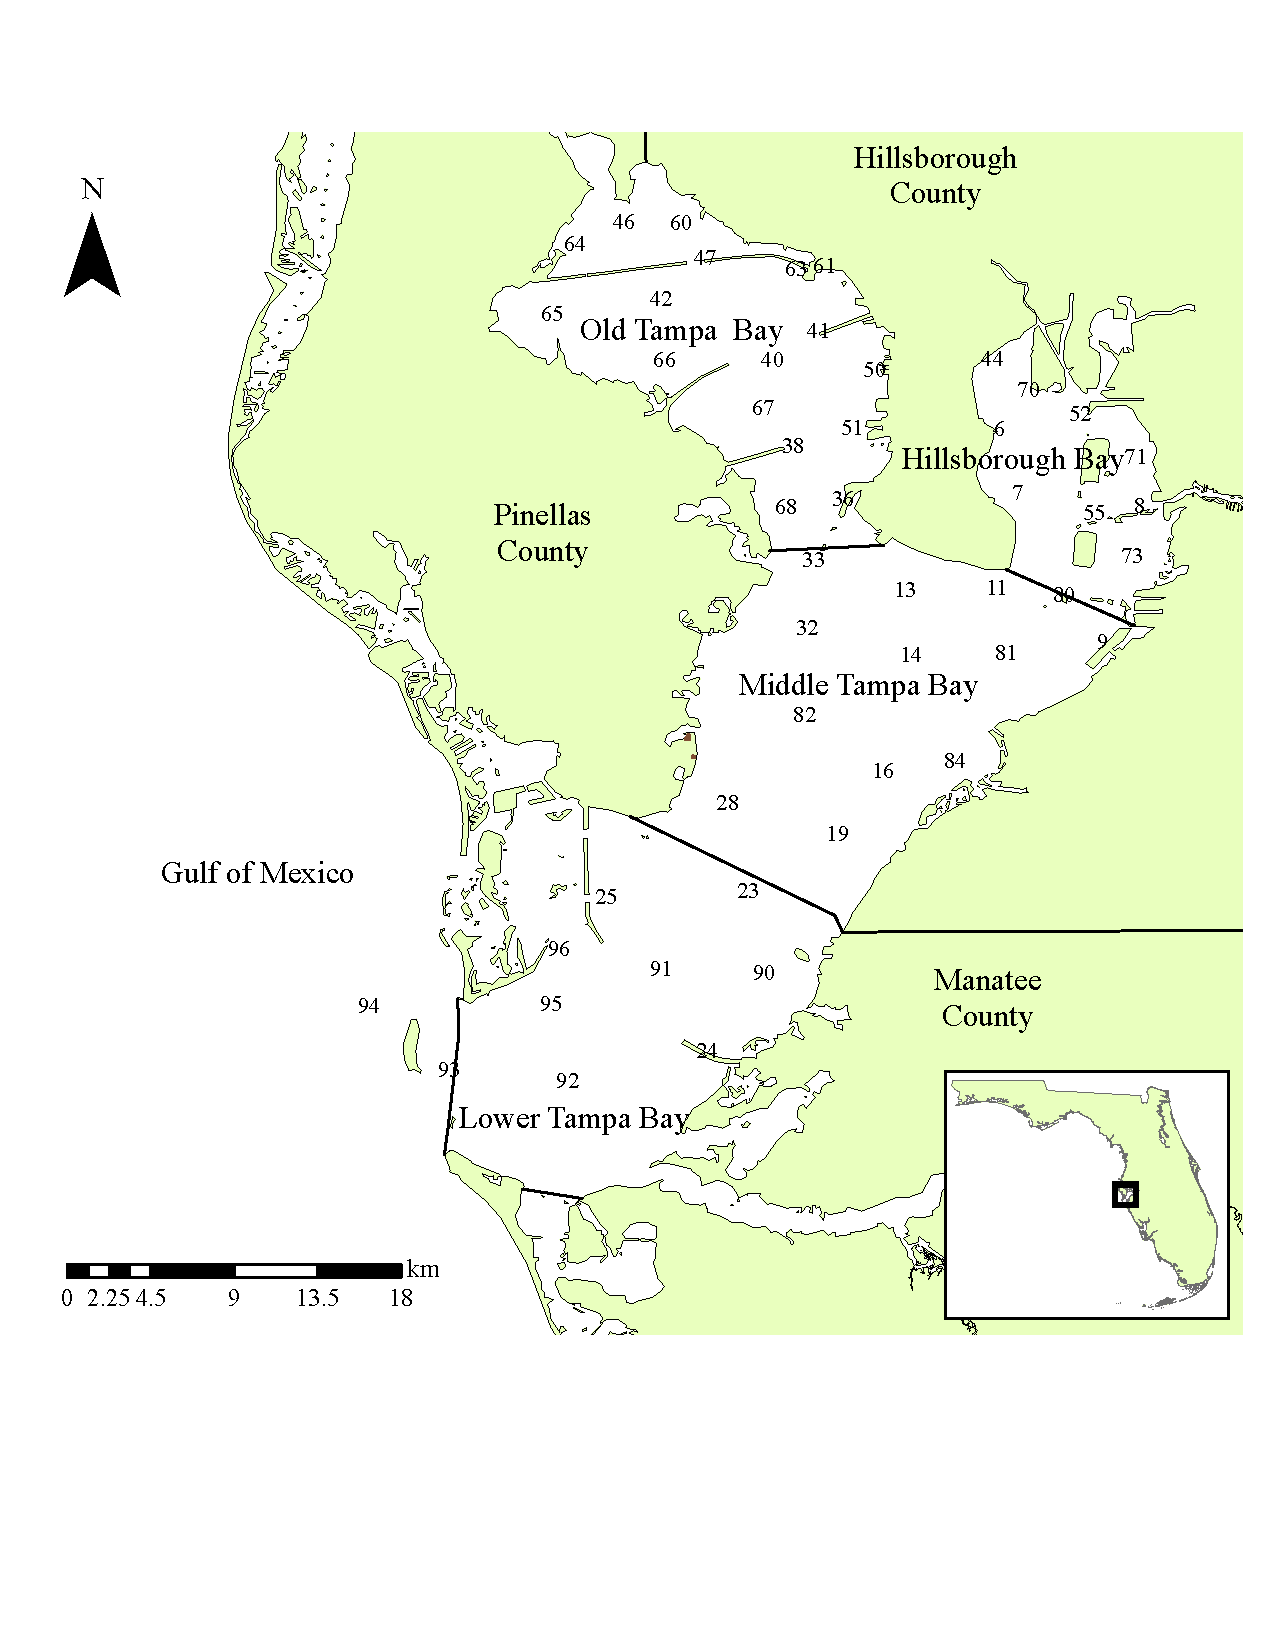
\includegraphics[width=0.9\textwidth]{figs/tb_map.pdf}
\caption{The Tampa Bay estuary located on the west coast of central Florida. The Bay is separated into four segments defined by chemical, physical, and geopolitical boundaries \cite{Lewis85}. Monthly water quality monitoring stations are also indicated by their identification number \cite{Boler01}.}
\label{fig:tb_map}
\end{figure}

%obs chlorophyll by year/month, uses station data

\begin{figure}
\centering
\subfloat[By year]{
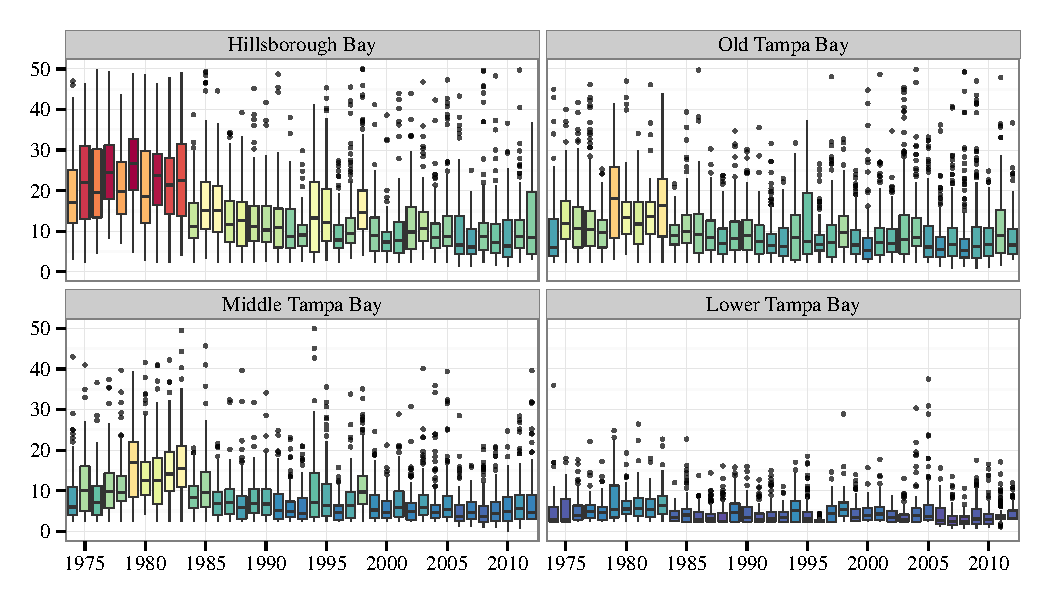
\includegraphics[width=\textwidth,page=1]{figs/obsyrmo.pdf}
\label{fig:obsyrmo1}
}

\subfloat[By month]{
\includegraphics[width=\textwidth,page=2]{figs/obsyrmo.pdf}
\label{fig:obsyrmo2}
}

\leavevmode\smash{\makebox[0pt]{\hspace{0em}% HORIZONTAL POSITION           
  \rotatebox[origin=l]{90}{\hspace{19em}% VERTICAL POSITION
    Chlorophyll-\textit{a} (\mugl)}%
}}\hspace{0pt plus 1filll}\null

\caption{Observed \ac{chl} data for Tampa Bay segments by \protect\subref{fig:obsyrmo1} year and \protect\subref{fig:obsyrmo2} month aggregations.  Each box is bisected and colored by the median.  Boxes represent the \ac{IQR} (25\textsuperscript{th} to 75\textsuperscript{th} percentile).  Outliers are present beyond whiskers (1.5$\cdot$\ac{IQR}) and were observed beyond 50 \mugl.}
\label{fig:obsyrmo}
\end{figure}

%weighting example
\begin{figure}[!ht]


{\centering 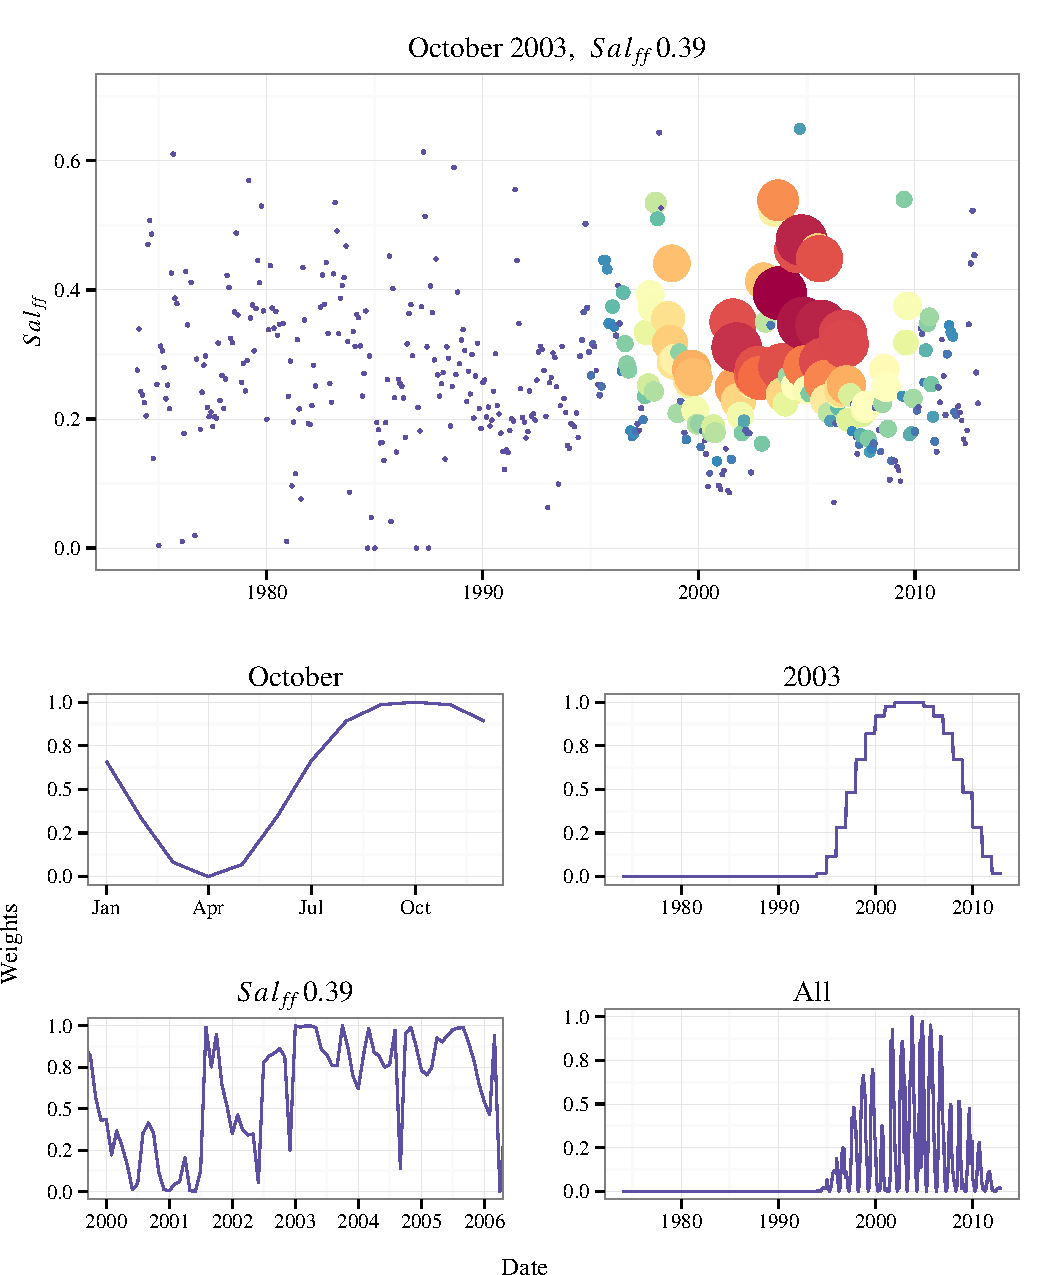
\includegraphics[width=6in]{M:/docs/manuscripts/tb_chl/figs/wtex} 

}

\caption[Example of weighting for one observation in Hillsborough Bay]{Example of weighting for one observation in Hillsborough Bay.  The top plot shows all data weighted for October 2003 when the proportion freshwater was 0.39.  Point size and color are in proportion to weights (small blue points = 0, large red points = 1).  The bottom plots show the individual weights for month, year, proportion freshwater, and all weights combined.\label{fig:wtex}}
\end{figure}



%predictions from model, all data
\begin{figure}[!ht]


{\centering 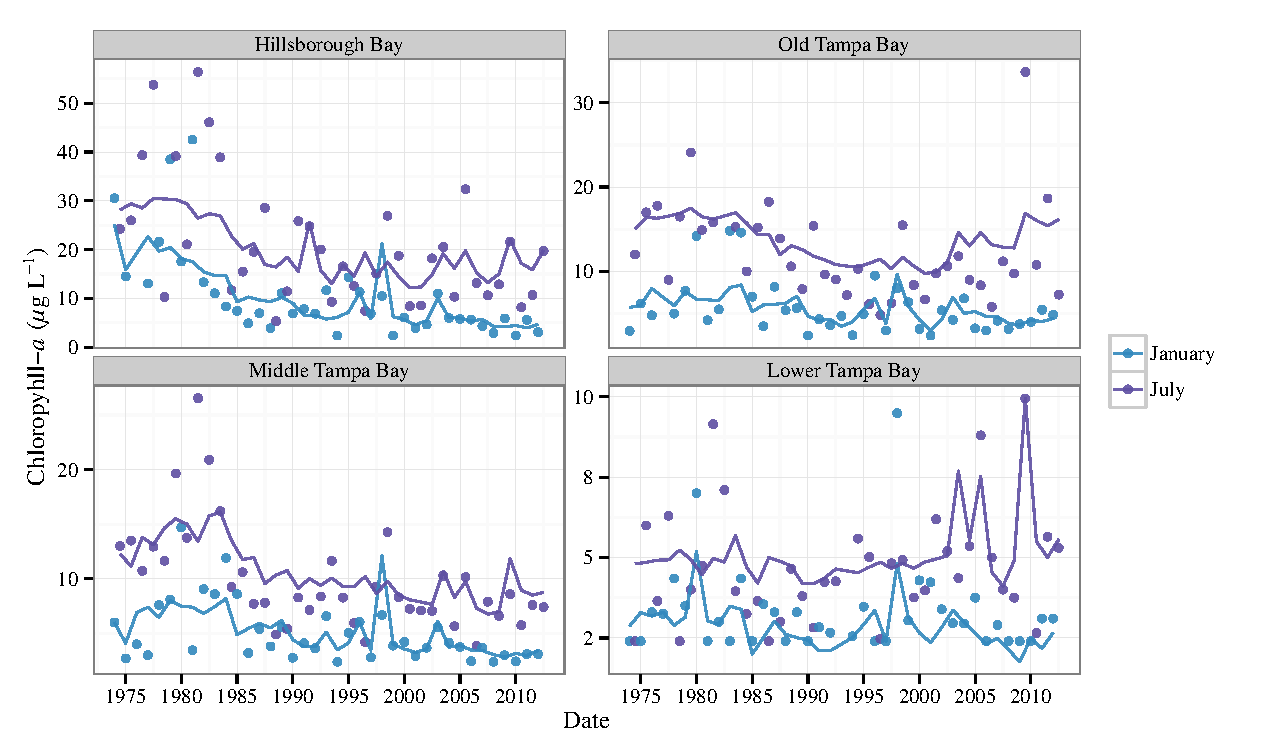
\includegraphics[width=6in]{M:/docs/manuscripts/tb_chl/figs/predobs} 

}

\caption[Predicted (lines) and observed (circles) \ac{chl} concentrations for Tampa Bay segments in January (dry season) and July (wet season) (see supplements for all months)]{Predicted (lines) and observed (circles) \ac{chl} concentrations for Tampa Bay segments in January (dry season) and July (wet season) (see supplements for all months).  Predicted values are for the weighted regression models fit through the median response.\label{fig:predobs}}
\end{figure}



\begin{figure}[!ht]


{\centering 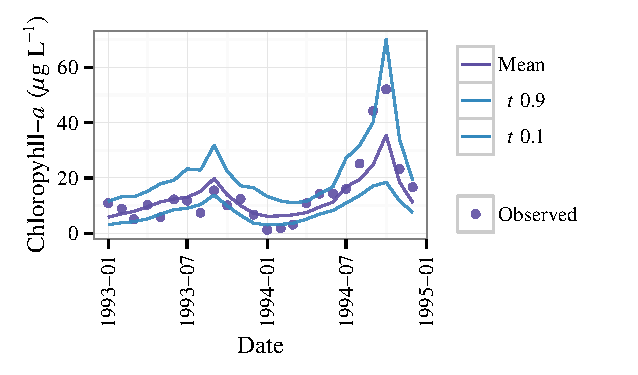
\includegraphics[width=3in]{M:/docs/manuscripts/tb_chl/figs/hbslice} 

}

\caption[Predicted and observed \ac{chl} concentrations for Hillsborough Bay for 1993 to 1995 illustrating variation in model fit based on observation date]{Predicted and observed \ac{chl} concentrations for Hillsborough Bay for 1993 to 1995 illustrating variation in model fit based on observation date. Predicted values are for the weighted regression models fit through the the 10\textsuperscript{th}, 50\textsuperscript{th}, and and 90\textsuperscript{th} percentile ($\tau$) distributions.\label{fig:hbslice}}
\end{figure}



\begin{figure}[!ht]


{\centering 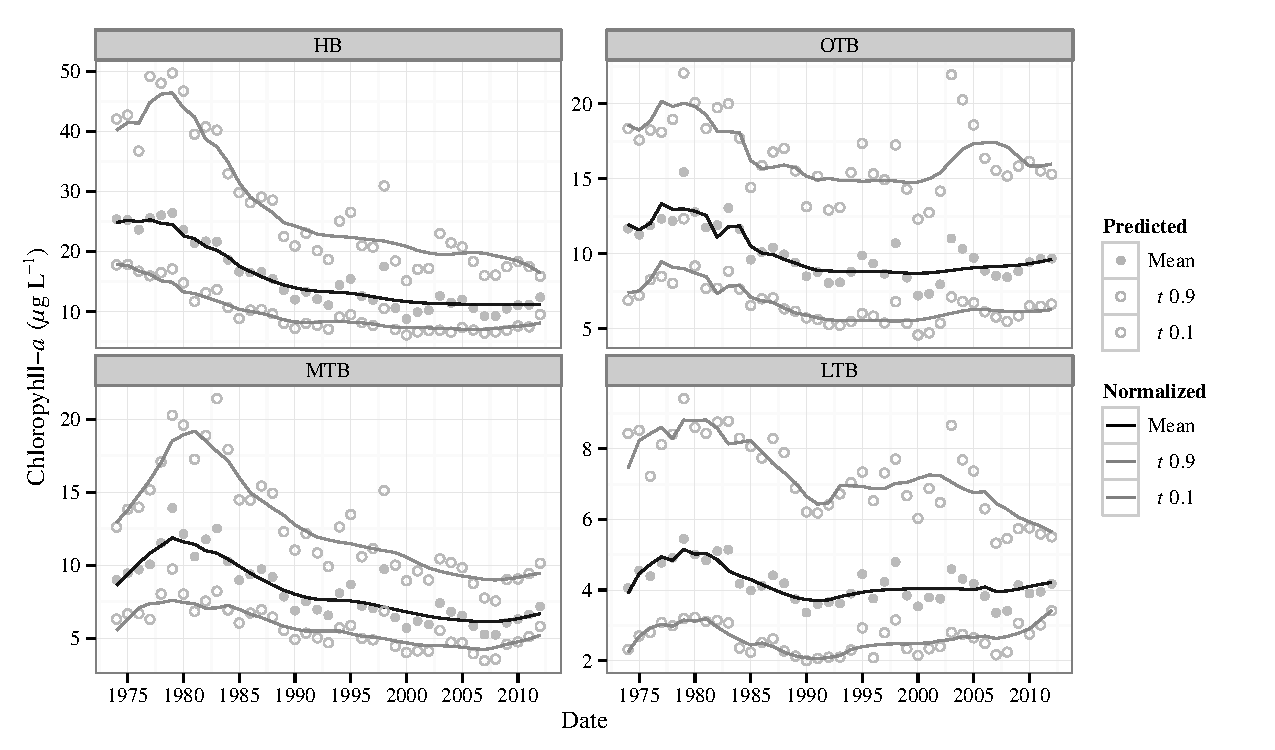
\includegraphics[width=6in]{M:/docs/manuscripts/tb_chl/figs/salnrm} 

}

\caption[Weighted regression predictions and salinity-normalized results aggregated by year for  the 10\textsuperscript{th}, 50\textsuperscript{th}, and 90\textsuperscript{th} quantile ($\tau$) distributions]{Weighted regression predictions and salinity-normalized results aggregated by year for  the 10\textsuperscript{th}, 50\textsuperscript{th}, and 90\textsuperscript{th} quantile ($\tau$) distributions.\label{fig:salnrm}}
\end{figure}



\begin{figure}[!ht]


{\centering 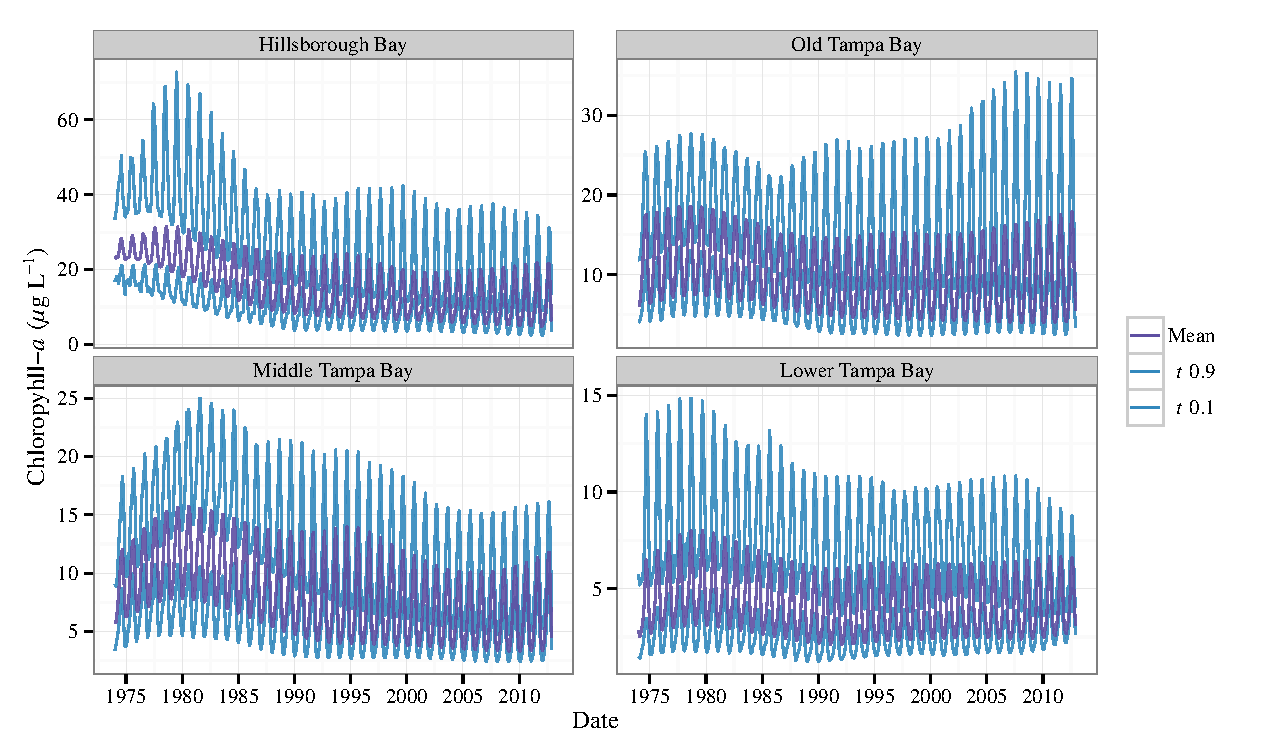
\includegraphics[width=6in]{M:/docs/manuscripts/tb_chl/figs/salnrm2} 

}

\caption[Salinity-normalized results for the 10\textsuperscript{th}, 50\textsuperscript{th}, and 90\textsuperscript{th} quantile ($\tau$) distributions]{Salinity-normalized results for the 10\textsuperscript{th}, 50\textsuperscript{th}, and 90\textsuperscript{th} quantile ($\tau$) distributions. Note changes in intra-annual variability by Bay segment.\label{fig:salnrm2}}
\end{figure}



\begin{figure}[!ht]


{\centering 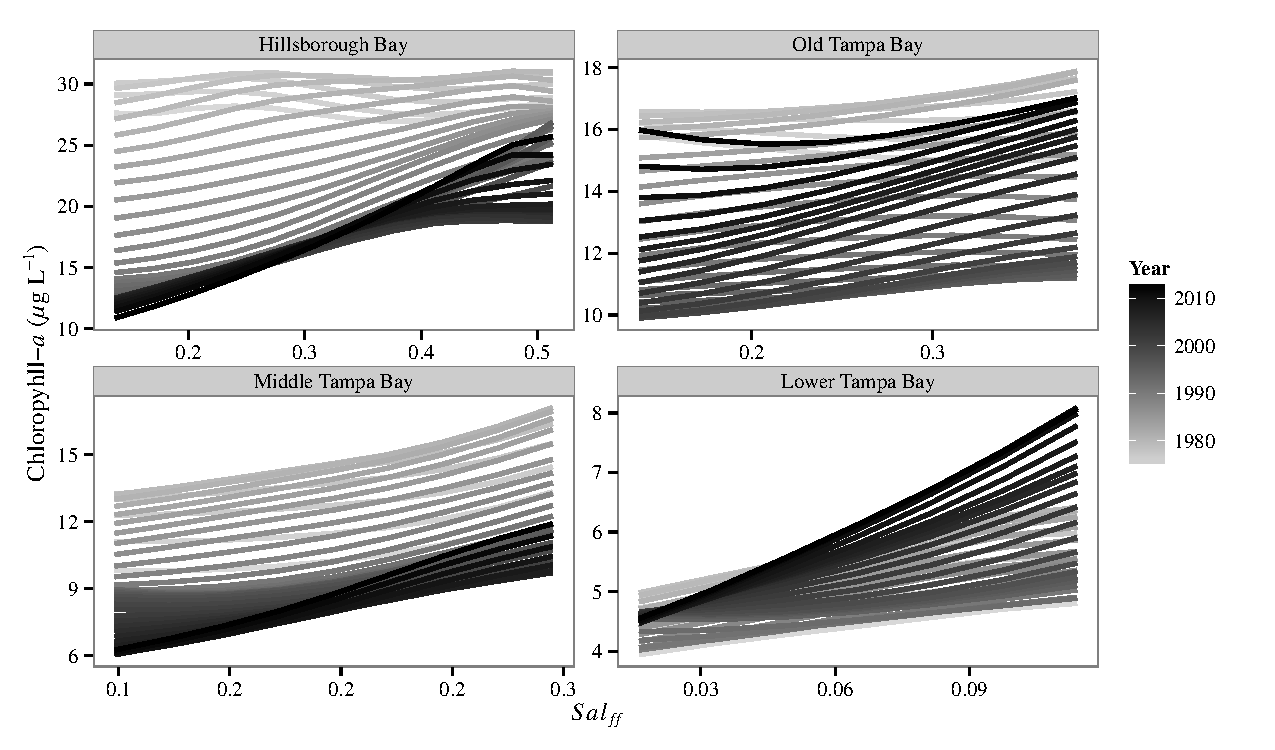
\includegraphics[width=6in]{M:/docs/manuscripts/tb_chl/figs/dyna} 

}

\caption[Variation in the relationship between \ac{chl} and salinity as fraction of freshwater ($Sal_{ff}$) across time series for Tampa Bay]{Variation in the relationship between \ac{chl} and salinity as fraction of freshwater ($Sal_{ff}$) across time series for Tampa Bay. Data are for July months to reduce seasonal variation. Only the median response models are shown.\label{fig:dyna}}
\end{figure}



\clearpage
\section{Supplementary material}

Please see the online repository (\href{https://github.com/fawda123/wtreg\_for\_estuaries}{https://github.com/fawda123/wtreg\_for\_estuaries}) for a current version of the adapted weighted regression approach for estuaries.  Note that the online version is in development and may not produce results that are identical to those in the manuscript. The corresponding author may be contacted directly with questions or comments.  

\beginsupplement
%predictions from model, all data
\begin{landscape}
\centering\vspace*{\fill}
\begin{figure}[!ht]


{\centering 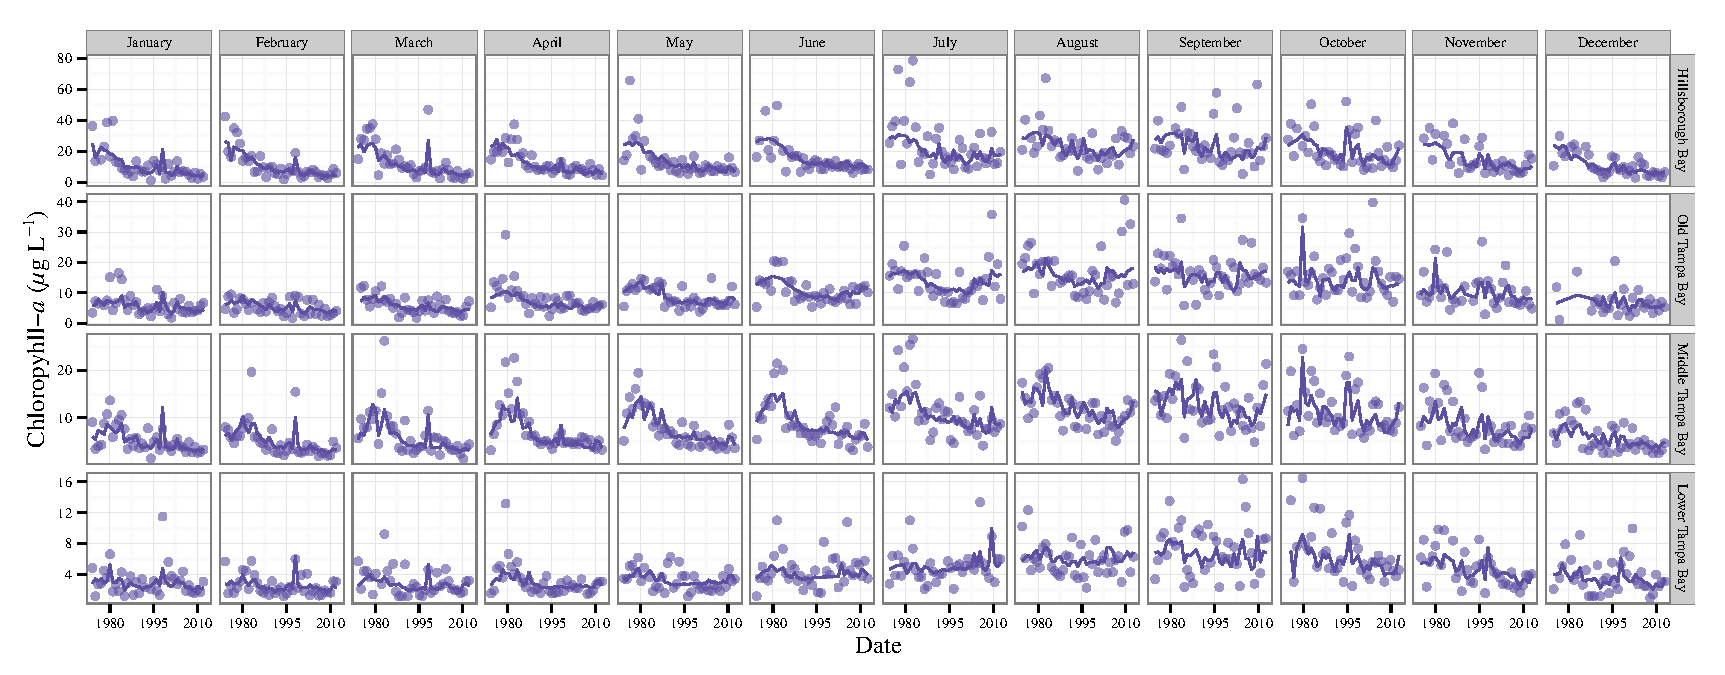
\includegraphics[width=9in]{M:/docs/manuscripts/tb_chl/figs/sup} 

}

\caption[Predicted (lines) and observed (circles) \ac{chl} concentrations for Tampa Bay segments by month]{Predicted (lines) and observed (circles) \ac{chl} concentrations for Tampa Bay segments by month.  Predicted values are for the weighted regression models fit through the median response.\label{fig:sup}}
\end{figure}


\vfill
\end{landscape}

\end{document}
